% =====================================================================
%  SRS-1 Datos — Especificación de requisitos (IEEE 830)
%  Compilar con pdfLaTeX (en Overleaf: Menu > Compiler > pdfLaTeX).
%  Fuente: Carlito (versión libre de Calibri, mismas métricas).
%  Carpeta figuras/: láminas de referencia (recortes de artículos CC BY).
% =====================================================================
\documentclass[11pt]{article}
\usepackage[letterpaper,left=3cm,right=3cm,top=2.5cm,bottom=2.5cm]{geometry}
\usepackage[utf8]{inputenc}
\usepackage[T1]{fontenc}
\usepackage[sfdefault,lf]{carlito}
\usepackage{textcomp}
\usepackage[spanish,es-nolayout,es-noshorthands,es-nodecimaldot,es-nopercent]{babel}
\usepackage{graphicx}
\usepackage[table]{xcolor}
\usepackage{array}
\usepackage{longtable}
\usepackage{enumitem}
\usepackage{titlesec}
\usepackage{caption}
\usepackage{xurl}
\urlstyle{same}
\usepackage{ragged2e}
\usepackage[hidelinks]{hyperref}

\definecolor{encabezado}{HTML}{D9E2F3}
\linespread{1.08}
\setlength{\parindent}{0pt}
\setlength{\parskip}{6pt}
\emergencystretch=2em
\pagestyle{plain}

\titleformat{\section}{\fontsize{13}{15.5}\selectfont\bfseries}{\thesection.}{0.6em}{}
\titlespacing*{\section}{0pt}{14pt}{6pt}
\titleformat{\subsection}{\normalsize\bfseries}{\thesubsection}{0.6em}{}
\titlespacing*{\subsection}{0pt}{10pt}{4pt}
\titleformat{\subsubsection}{\normalsize\bfseries\itshape}{\thesubsubsection}{0.6em}{}
\titlespacing*{\subsubsection}{0pt}{8pt}{3pt}
\setcounter{tocdepth}{2}

\captionsetup{font={small},labelfont=bf,textfont=it,labelsep=period,justification=raggedright,singlelinecheck=false}
\captionsetup[table]{name=Tabla,position=top,skip=4pt}
\captionsetup[figure]{name=Figura,position=bottom,skip=4pt}
\setlength{\LTcapwidth}{\linewidth}
\setlength{\LTpre}{6pt}
\setlength{\LTpost}{4pt}
\setlength{\tabcolsep}{0.123cm}
\renewcommand{\arraystretch}{1.15}
\newcommand{\nota}[1]{\par\vspace{-4pt}{\fontsize{9}{11}\selectfont\justifying #1\par}\vspace{2pt}}

\begin{document}

% ------------------------------------------------------------------ Portada
\begin{titlepage}
\centering
\vspace*{2.5cm}
{\Large\bfseries Especificación de requisitos de software\par}
\vspace{0.4cm}
{\large Conforme al estándar IEEE Std 830-1998\par}
\vspace{1.6cm}
{\LARGE\bfseries SRS-1: Conjunto de datos de imágenes\\[4pt] del tallo principal del aguacate\par}
\vspace{1.4cm}
{\large Proyecto: Smart Agriculture\par}
\vspace{0.3cm}
{\normalsize Aplicación móvil para detectar alteraciones visibles en el tallo del aguacate\par}
\vfill
{\normalsize
Autor: Ariel Llumiquinga\\
Tutora: Ing. Doris Chicaiza\\[6pt]
Laboratorio de Investigación de Software\\
Departamento de Ciencias de la Computación\\
Universidad de las Fuerzas Armadas ESPE\\[10pt]
Versión 0.1 (borrador) · 7 de octubre de 2026\par}
\end{titlepage}

\section*{Ficha del documento}
{\small
\begin{longtable}{|>{\RaggedRight\arraybackslash}p{2.29cm}|>{\RaggedRight\arraybackslash}p{1.53cm}|>{\RaggedRight\arraybackslash}p{3.43cm}|>{\RaggedRight\arraybackslash}p{3.43cm}|>{\RaggedRight\arraybackslash}p{3.43cm}|}
\caption{Control de versiones}\\
\hline
\rowcolor{encabezado}\textbf{Fecha} & \textbf{Versión} & \textbf{Autor} & \textbf{Revisora} & \textbf{Estado} \\ \hline
\endfirsthead
\hline
\rowcolor{encabezado}\textbf{Fecha} & \textbf{Versión} & \textbf{Autor} & \textbf{Revisora} & \textbf{Estado} \\ \hline
\endhead
07/10/2026 & 0.1 & Ariel Llumiquinga & Ing. Doris Chicaiza & Borrador para revisión \\ \hline
\end{longtable}}
\textbf{Cómo usar este documento.} Este SRS es autosuficiente: con él se puede construir el conjunto de datos sin consultar otros documentos. La \textbf{sección 3} dice \textbf{qué} debe cumplir el conjunto (requisitos funcionales RF y no funcionales RNF); el \textbf{Anexo A} dice \textbf{cómo} hacerlo paso a paso; el \textbf{Anexo B} enseña a reconocer cada clase con fotos de referencia; los \textbf{Anexos C y D} traen el diccionario de datos y los formatos de campo; y el \textbf{Anexo E}, las metas y el tiempo de captura.

\tableofcontents
\clearpage
\section{Introducción}
\subsection{Propósito}
Este documento especifica los requisitos del \textbf{conjunto de datos de imágenes del tallo principal del aguacate} que se construirá en el proyecto Smart Agriculture. El conjunto servirá para entrenar, validar y probar un modelo de inteligencia artificial que se ejecutará en una aplicación móvil Android sin conexión.

Está dirigido a: el autor, que diseña, captura y etiqueta el conjunto; la persona del grupo que capture las fotos en campo; la tutora, que lo revisa y valida; y el equipo que desarrollará el modelo, que recibirá el conjunto.

\subsection{Alcance}
\textbf{Producto:} Conjunto de datos de imágenes del tallo principal del aguacate, versión 1.0. Comprende las fotografías originales, sus etiquetas, sus metadatos y su partición en conjuntos de desarrollo y prueba.

{\small
\begin{longtable}{|>{\RaggedRight\arraybackslash}p{7.43cm}|>{\RaggedRight\arraybackslash}p{7.43cm}|}
\caption{Qué incluye y qué no incluye el conjunto de datos}\\
\hline
\rowcolor{encabezado}\textbf{Incluye} & \textbf{No incluye} \\ \hline
\endfirsthead
\hline
\rowcolor{encabezado}\textbf{Incluye} & \textbf{No incluye} \\ \hline
\endhead
\textbullet~Fotos del tallo principal: cuello, zona de injerto, fuste y cruz.\newline \textbullet~Árboles jóvenes y adultos de fincas de Sigchos (Ecuador).\newline \textbullet~Troncos sanos y con alteraciones visibles desde fuera.\newline \textbullet~Fotos tomadas con teléfono y luz natural.\newline \textbullet~Etiquetas por tipo de síntoma, metadatos y partición. & \textbullet~Raíz, ramas sobre la cruz, hojas y frutos.\newline \textbullet~Síntomas internos (requieren cortar).\newline \textbullet~Identificación de la especie del patógeno.\newline \textbullet~Severidad como resultado del modelo.\newline \textbullet~Localización de la lesión con cajas o contornos.\newline \textbullet~Preprocesamiento y aumento de datos (son del modelo, SRS-2). \\ \hline
\end{longtable}}
\textbf{Beneficio.} La revisión sistemática del proyecto encontró que no existen sistemas de IA ni conjuntos de imágenes para el tallo del aguacate, ni estudios de Ecuador. Este conjunto será el primero para ese fin.

\subsection{Personal involucrado}
{\small
\begin{longtable}{|>{\RaggedRight\arraybackslash}p{3.91cm}|>{\RaggedRight\arraybackslash}p{10.95cm}|}
\caption{Personal involucrado: Ariel Llumiquinga}\\
\hline
\rowcolor{encabezado}\textbf{Campo} & \textbf{Detalle} \\ \hline
\endfirsthead
\hline
\rowcolor{encabezado}\textbf{Campo} & \textbf{Detalle} \\ \hline
\endhead
Nombre & Ariel Llumiquinga \\ \hline
Rol & Autor; analista de requisitos y etiquetador \\ \hline
Categoría profesional & Estudiante de prácticas preprofesionales, Ingeniería de Software \\ \hline
Responsabilidades & Especificar los requisitos, dirigir la prueba piloto, depurar, etiquetar, partir y entregar el conjunto \\ \hline
Información de contacto & — \\ \hline
\end{longtable}}
{\small
\begin{longtable}{|>{\RaggedRight\arraybackslash}p{3.91cm}|>{\RaggedRight\arraybackslash}p{10.95cm}|}
\caption{Personal involucrado: Ing. Doris Chicaiza}\\
\hline
\rowcolor{encabezado}\textbf{Campo} & \textbf{Detalle} \\ \hline
\endfirsthead
\hline
\rowcolor{encabezado}\textbf{Campo} & \textbf{Detalle} \\ \hline
\endhead
Nombre & Ing. Doris Chicaiza \\ \hline
Rol & Tutora y revisora \\ \hline
Categoría profesional & Docente, Departamento de Ciencias de la Computación \\ \hline
Responsabilidades & Revisar y validar este documento y la versión base del conjunto \\ \hline
Información de contacto & — \\ \hline
\end{longtable}}
{\small
\begin{longtable}{|>{\RaggedRight\arraybackslash}p{3.91cm}|>{\RaggedRight\arraybackslash}p{10.95cm}|}
\caption{Personal involucrado: Docente del proyecto (por confirmar)}\\
\hline
\rowcolor{encabezado}\textbf{Campo} & \textbf{Detalle} \\ \hline
\endfirsthead
\hline
\rowcolor{encabezado}\textbf{Campo} & \textbf{Detalle} \\ \hline
\endhead
Nombre & Docente del proyecto (por confirmar) \\ \hline
Rol & Enlace con las fincas \\ \hline
Categoría profesional & Docente \\ \hline
Responsabilidades & Gestionar el acceso a las fincas y el consentimiento de los dueños \\ \hline
Información de contacto & — \\ \hline
\end{longtable}}
{\small
\begin{longtable}{|>{\RaggedRight\arraybackslash}p{3.91cm}|>{\RaggedRight\arraybackslash}p{10.95cm}|}
\caption{Personal involucrado: Fotógrafo designado (por confirmar)}\\
\hline
\rowcolor{encabezado}\textbf{Campo} & \textbf{Detalle} \\ \hline
\endfirsthead
\hline
\rowcolor{encabezado}\textbf{Campo} & \textbf{Detalle} \\ \hline
\endhead
Nombre & Fotógrafo designado (por confirmar) \\ \hline
Rol & Captura en campo \\ \hline
Categoría profesional & Miembro del grupo de desarrollo \\ \hline
Responsabilidades & Tomar las fotos y llenar las hojas de campo según este documento \\ \hline
Información de contacto & — \\ \hline
\end{longtable}}
\subsection{Definiciones, acrónimos y abreviaturas}
{\small
\begin{longtable}{|>{\RaggedRight\arraybackslash}p{3.91cm}|>{\RaggedRight\arraybackslash}p{10.95cm}|}
\caption{Términos de la planta y de los síntomas}\\
\hline
\rowcolor{encabezado}\textbf{Término} & \textbf{Significado} \\ \hline
\endfirsthead
\hline
\rowcolor{encabezado}\textbf{Término} & \textbf{Significado} \\ \hline
\endhead
Tallo principal (tronco) & Eje leñoso único del árbol, desde el cuello hasta la cruz. \\ \hline
Cuello & Base del tronco, en contacto con el suelo. \\ \hline
Zona de injerto & Franja donde se unen el portainjerto (planta de abajo) y la variedad (planta de arriba). \\ \hline
Fuste & Tramo del tronco entre el injerto y la cruz. \\ \hline
Cruz & Punto donde nace la primera rama principal; límite superior de las fotos. \\ \hline
Cancro & Lesión de la corteza, de color oscuro, con o sin hundimiento, a veces con exudado. \\ \hline
Exudado & Savia que sale de la corteza; en los cancros puede secar en un polvo blanco (perseitol). No siempre indica enfermedad. \\ \hline
Necrosis & Tejido muerto, de color oscuro. \\ \hline
Corteza friable & Corteza quebradiza que se levanta o desprende. \\ \hline
Coinfección & Varios patógenos en la misma planta. \\ \hline
\end{longtable}}
{\small
\begin{longtable}{|>{\RaggedRight\arraybackslash}p{3.91cm}|>{\RaggedRight\arraybackslash}p{10.95cm}|}
\caption{Términos de datos y acrónimos}\\
\hline
\rowcolor{encabezado}\textbf{Término} & \textbf{Significado} \\ \hline
\endfirsthead
\hline
\rowcolor{encabezado}\textbf{Término} & \textbf{Significado} \\ \hline
\endhead
Conjunto de datos & Fotos, etiquetas, metadatos y partición que se entregan al modelo. \\ \hline
Clase / etiqueta & Categoría que el modelo aprende (p. ej., “Cancro seco”); la etiqueta es la clase asignada a una foto. \\ \hline
Metadatos & Datos de contexto de cada foto: árbol, finca, fecha, luz, teléfono, etc. \\ \hline
Partición & División del conjunto en desarrollo (entrenamiento y validación) y prueba. \\ \hline
Fuga de datos & Error en que fotos del mismo árbol quedan en entrenamiento y prueba, lo que infla los resultados. \\ \hline
Coeficiente Kappa & Medida de cuánto coinciden dos etiquetados más allá del azar: 1 es acuerdo total; 0, el que daría el azar. \\ \hline
RF / RNF & Requisito funcional / requisito no funcional. \\ \hline
SRS & Especificación de requisitos de software. SRS-1: datos; SRS-2: modelo de IA; SRS-3: aplicación móvil. \\ \hline
IA & Inteligencia artificial. \\ \hline
MP & Megapíxeles (resolución de la cámara). \\ \hline
JPG / CSV & Formato de imagen / formato de tabla de texto separada por comas. \\ \hline
EXIF & Datos que el teléfono guarda dentro de cada foto (fecha, modelo, resolución, ubicación). \\ \hline
GPS & Ubicación por satélite del teléfono. \\ \hline
SLR & Revisión sistemática de literatura del proyecto. \\ \hline
Act. & Actividad del itinerario de prácticas (28 actividades). \\ \hline
\end{longtable}}
\subsection{Referencias}
{\small
\begin{longtable}{|>{\RaggedRight\arraybackslash}p{2.04cm}|>{\RaggedRight\arraybackslash}p{4.27cm}|>{\RaggedRight\arraybackslash}p{4.09cm}|>{\RaggedRight\arraybackslash}p{1.67cm}|>{\RaggedRight\arraybackslash}p{2.04cm}|}
\caption{Documentos del proyecto}\\
\hline
\rowcolor{encabezado}\textbf{Referencia} & \textbf{Título} & \textbf{Ruta} & \textbf{Fecha} & \textbf{Autor} \\ \hline
\endfirsthead
\hline
\rowcolor{encabezado}\textbf{Referencia} & \textbf{Título} & \textbf{Ruta} & \textbf{Fecha} & \textbf{Autor} \\ \hline
\endhead
SLR v1 & Revisión sistemática: enfermedades del tallo del aguacate e IA & \nolinkurl{SLR_SmartAgriculture/05_Redaccion_SLR} & 06/10/2026 & A. Llumiquinga \\ \hline
DS-01 a DS-10 & Documentos de soporte del SRS-1 (análisis detallado) & \nolinkurl{SRS/00_SRS_Datos} & 06/10/2026 & A. Llumiquinga \\ \hline
Control & Registro de decisiones y pendientes del SRS-1 & \nolinkurl{SRS/00_SRS_Datos/Control_SRS1_Datos.xlsx} & 07/10/2026 & A. Llumiquinga \\ \hline
IEEE 830 & Plantilla de especificación de requisitos & \nolinkurl{SRS/02_SRS_App} & 2017 & Plantilla del proyecto \\ \hline
\end{longtable}}
Las fuentes científicas citadas se listan en la Bibliografía, al final. Todas forman parte de la carpeta de fuentes del proyecto.

\section{Descripción general}
\subsection{Perspectiva del producto}
El conjunto de datos es el primer eslabón del sistema: \textbf{SRS-1 (datos) $\rightarrow$ SRS-2 (modelo de IA) $\rightarrow$ SRS-3 (aplicación móvil)}. Las clases definidas aquí son las salidas del modelo, y la entrega de la versión 1.0 es la entrada del SRS-2. Por eso, un cambio de clases obliga a revisar el modelo y la aplicación.

\subsection{Funcionalidad del producto}
{\small
\begin{longtable}{|>{\RaggedRight\arraybackslash}p{2.84cm}|>{\RaggedRight\arraybackslash}p{5.67cm}|>{\RaggedRight\arraybackslash}p{1.7cm}|>{\RaggedRight\arraybackslash}p{4.16cm}|}
\caption{Etapas de construcción del conjunto de datos}\\
\hline
\rowcolor{encabezado}\textbf{Etapa} & \textbf{Qué se hace} & \textbf{Actividad} & \textbf{Requisitos} \\ \hline
\endfirsthead
\hline
\rowcolor{encabezado}\textbf{Etapa} & \textbf{Qué se hace} & \textbf{Actividad} & \textbf{Requisitos} \\ \hline
\endhead
1. Preparación & Consentimiento, configuración del teléfono, materiales y formatos & Act. 14 & RNF-03, RNF-25 \\ \hline
2. Captura & Prueba piloto, selección de árboles, fotos y hojas de campo & Act. 15 & RF-01, RF-06 a RF-14, RNF-01 a RNF-06 \\ \hline
3. Depuración & Renombrar, revisar calidad, descartar y quitar duplicados & Act. 16 & RF-15, RF-16, RF-21, RF-22, RNF-07, RNF-08 \\ \hline
4. Etiquetado & Etiquetar, registrar dudas, controlar la consistencia y decidir el nivel de clases & Act. 16 & RF-02 a RF-05, RF-17 a RF-20, RNF-13 a RNF-15 \\ \hline
5. Partición y entrega & Partir por grupos, generar carpetas, informes y manifiesto & Act. 17 & RF-24 a RF-28, RNF-16 a RNF-22 \\ \hline
\end{longtable}}
\subsection{Características de los usuarios}
{\small
\begin{longtable}{|>{\RaggedRight\arraybackslash}p{3.91cm}|>{\RaggedRight\arraybackslash}p{10.95cm}|}
\caption{Usuario: Autor (etiquetador)}\\
\hline
\rowcolor{encabezado}\textbf{Campo} & \textbf{Detalle} \\ \hline
\endfirsthead
\hline
\rowcolor{encabezado}\textbf{Campo} & \textbf{Detalle} \\ \hline
\endhead
Tipo de usuario & Autor (etiquetador) \\ \hline
Formación & Estudiante de Ingeniería de Software con la investigación del tallo \\ \hline
Habilidades & Reconocer las clases con el Anexo B; manejar hojas de cálculo y scripts \\ \hline
Actividades & Dirigir la prueba piloto, depurar, etiquetar, partir y entregar \\ \hline
\end{longtable}}
{\small
\begin{longtable}{|>{\RaggedRight\arraybackslash}p{3.91cm}|>{\RaggedRight\arraybackslash}p{10.95cm}|}
\caption{Usuario: Fotógrafo designado}\\
\hline
\rowcolor{encabezado}\textbf{Campo} & \textbf{Detalle} \\ \hline
\endfirsthead
\hline
\rowcolor{encabezado}\textbf{Campo} & \textbf{Detalle} \\ \hline
\endhead
Tipo de usuario & Fotógrafo designado \\ \hline
Formación & Miembro del grupo; puede no conocer la investigación \\ \hline
Habilidades & Usar el teléfono y seguir el Anexo A \\ \hline
Actividades & Tomar las fotos y llenar las hojas de campo \\ \hline
\end{longtable}}
{\small
\begin{longtable}{|>{\RaggedRight\arraybackslash}p{3.91cm}|>{\RaggedRight\arraybackslash}p{10.95cm}|}
\caption{Usuario: Equipo del modelo}\\
\hline
\rowcolor{encabezado}\textbf{Campo} & \textbf{Detalle} \\ \hline
\endfirsthead
\hline
\rowcolor{encabezado}\textbf{Campo} & \textbf{Detalle} \\ \hline
\endhead
Tipo de usuario & Equipo del modelo \\ \hline
Formación & Desarrolladores del SRS-2 \\ \hline
Habilidades & Aprendizaje profundo \\ \hline
Actividades & Usar la entrega 1.0 respetando RNF-22 \\ \hline
\end{longtable}}
\subsection{Restricciones}
\begin{itemize}[leftmargin=1.2em,itemsep=2pt,topsep=2pt]
\item No hay un experto fitopatólogo que valide clases ni etiquetas: todo se basa en la literatura del proyecto.
\item No habrá visita previa a las fincas; se irá solo a capturar.
\item La captura está prevista en 2 días (28 y 29/10, Act. 15); una ampliación está por conversar.
\item Solo se usan las fuentes recopiladas por el autor.
\item Solo el tallo principal.
\item La captura podría hacerla otra persona del grupo.
\item Los agricultores de Sigchos usan sobre todo teléfonos de gama baja.
\item Una sola época del año (octubre).
\item Prácticas de 240 horas en total.
\end{itemize}
\subsection{Suposiciones y dependencias}
{\small
\begin{longtable}{|>{\RaggedRight\arraybackslash}p{6.73cm}|>{\RaggedRight\arraybackslash}p{2.31cm}|>{\RaggedRight\arraybackslash}p{5.58cm}|}
\caption{Suposiciones}\\
\hline
\rowcolor{encabezado}\textbf{Suposición} & \textbf{Estado} & \textbf{Si no se cumple} \\ \hline
\endfirsthead
\hline
\rowcolor{encabezado}\textbf{Suposición} & \textbf{Estado} & \textbf{Si no se cumple} \\ \hline
\endhead
Se accederá a más de 3 fincas por medio del docente del proyecto & Confirmada & Reducir el muestreo o pedir más días \\ \hline
Habrá árboles con síntomas visibles en el tallo & Sin verificar & Fusionar clases (RF-05) \\ \hline
Los dueños darán su consentimiento & Sin verificar & No fotografiar esa finca \\ \hline
Los síntomas de Sigchos se parecerán a los de la literatura & Sin verificar & Usar No concluyente y declarar la limitación \\ \hline
Habrá luz natural suficiente & Probable & Registrar la luz y descartar las fotos no válidas \\ \hline
\end{longtable}}
\textbf{Dependencias:} el modelo (SRS-2) depende de las clases de este documento; el protocolo de captura de la Act. 14 aplica este documento; el acceso a las fincas depende del docente del proyecto.

\subsection{Evolución previsible del sistema}
El conjunto podrá crecer con más fincas, otras épocas del año, otros teléfonos y nuevas clases si en el futuro un experto valida las etiquetas. Por eso los nombres, las carpetas y las tablas admiten ampliaciones sin rehacer lo existente.

\section{Requisitos específicos}
\subsection{Requisitos comunes de las interfaces}
\subsubsection{Interfaces de usuario}
\begin{itemize}[leftmargin=1.2em,itemsep=2pt,topsep=2pt]
\item \textbf{Hojas de campo} (impresas o en el teléfono): hoja de finca y hoja de árbol (Anexo D).
\item \textbf{Tabla de etiquetas} en una hoja de cálculo: una fila por imagen con etiqueta, síntoma secundario, caso dudoso aplicado, seguridad, sesión, fecha y versión de la guía.
\item \textbf{Guía rápida de campo}: resumen del Anexo B que lleva quien captura.
\end{itemize}
\subsubsection{Interfaces de hardware}
\begin{itemize}[leftmargin=1.2em,itemsep=2pt,topsep=2pt]
\item Teléfono principal con cámara de 12 MP o más, GPS y brújula (RNF-01, RNF-03).
\item Teléfono secundario de gama baja, si existe (RNF-02).
\item Tarjetas de identificación, regla o tarjeta de tamaño conocido y cinta métrica.
\item Computador del autor, disco externo y almacenamiento del laboratorio para las copias (RNF-19).
\end{itemize}
\subsubsection{Interfaces de software}
\textbf{Entrega al equipo del modelo (SRS-2).} Propósito: que el modelo use el conjunto sin consultar otros documentos. Contenido y formato:

{\small
\begin{longtable}{|>{\RaggedRight\arraybackslash}p{3.32cm}|>{\RaggedRight\arraybackslash}p{11.53cm}|}
\caption{Contenido de la entrega 1.0}\\
\hline
\rowcolor{encabezado}\textbf{Elemento} & \textbf{Contenido y formato} \\ \hline
\endfirsthead
\hline
\rowcolor{encabezado}\textbf{Elemento} & \textbf{Contenido y formato} \\ \hline
\endhead
Imágenes & JPG originales válidas, sin ubicación en sus datos internos, en carpetas \nolinkurl{nivel/conjunto/clase} (p. ej., \nolinkurl{nivel_C/desarrollo/sano/}). \\ \hline
Lista de clases & Nombre, carpeta y definición de cada clase del nivel entregado. \\ \hline
Tablas CSV & imágenes, etiquetas finales, árboles, lesiones, niveles y partición, sin datos sensibles. \\ \hline
Partición & Conjunto (desarrollo, prueba o prueba externa) y pliegue (1 a 5) de cada árbol; semilla usada. \\ \hline
Informes & Depuración, etiquetado (Kappa), conteos y partición. \\ \hline
Manifiesto & Suma SHA-256 de cada archivo y conteos. \\ \hline
Limitaciones & Lista declarada (RNF-27). \\ \hline
\end{longtable}}
\textbf{El equipo del modelo deberá:} aplicar el aumento de datos y la normalización solo en entrenamiento (RNF-22); definir el umbral de confianza que produce el resultado “no concluyente” de la app; reponderar si el balance supera 3 a 1; reportar resultados por grupo de edad, teléfono y luz; y especificar el preprocesamiento (tamaño y normalización).

\subsubsection{Interfaces de comunicación}
No aplica: la captura y las copias se hacen sin conexión, copiando archivos.

\subsection{Requisitos funcionales}
{\small
\begin{longtable}{|>{\RaggedRight\arraybackslash}p{2.27cm}|>{\RaggedRight\arraybackslash}p{6.05cm}|>{\RaggedRight\arraybackslash}p{3.02cm}|>{\RaggedRight\arraybackslash}p{3.02cm}|}
\caption{Resumen de requisitos funcionales}\\
\hline
\rowcolor{encabezado}\textbf{No. de requisito} & \textbf{Nombre de requisito} & \textbf{Prioridad} & \textbf{Responsable} \\ \hline
\endfirsthead
\hline
\rowcolor{encabezado}\textbf{No. de requisito} & \textbf{Nombre de requisito} & \textbf{Prioridad} & \textbf{Responsable} \\ \hline
\endhead
RF-01 & Alcance de las imágenes & Alta / Esencial & Fotógrafo y autor \\ \hline
RF-02 & Clases del conjunto de datos & Alta / Esencial & Autor \\ \hline
RF-03 & Una sola etiqueta por imagen & Alta / Esencial & Autor \\ \hline
RF-04 & Tratamiento de “No concluyente” & Alta / Esencial & Autor \\ \hline
RF-05 & Niveles de clases según las imágenes obtenidas & Alta / Esencial & Autor \\ \hline
RF-06 & Árboles de distintas edades & Media / Deseado & Fotógrafo \\ \hline
RF-07 & Tipos de fotografía & Alta / Esencial & Fotógrafo \\ \hline
RF-08 & Fotografías mínimas por árbol & Alta / Esencial & Fotógrafo \\ \hline
RF-09 & Fotografías completas por árbol & Media / Deseado & Fotógrafo \\ \hline
RF-10 & Identificación de árboles y fotos & Alta / Esencial & Fotógrafo \\ \hline
RF-11 & Hoja de campo & Alta / Esencial & Fotógrafo \\ \hline
RF-12 & Prueba piloto & Alta / Esencial & Autor \\ \hline
RF-13 & Selección de árboles en cada finca & Alta / Esencial & Fotógrafo \\ \hline
RF-14 & Árboles sanos pareados & Media / Deseado & Fotógrafo \\ \hline
RF-15 & Depuración de imágenes & Alta / Esencial & Autor \\ \hline
RF-16 & Eliminación de duplicados & Alta / Esencial & Autor \\ \hline
RF-17 & Etiquetado con la guía & Alta / Esencial & Autor \\ \hline
RF-18 & Registro de dudas & Alta / Esencial & Autor \\ \hline
RF-19 & Doble etiquetado ciego & Alta / Esencial & Autor \\ \hline
RF-20 & Severidad por árbol & Media / Deseado & Autor \\ \hline
RF-21 & Tablas de metadatos & Alta / Esencial & Autor \\ \hline
RF-22 & Nombres de archivo y carpetas & Alta / Esencial & Autor \\ \hline
RF-23 & Medidas opcionales & Baja / Opcional & Fotógrafo \\ \hline
RF-24 & Partición por grupo & Alta / Esencial & Autor \\ \hline
RF-25 & Esquema de partición & Alta / Esencial & Autor \\ \hline
RF-26 & Prueba externa & Baja / Opcional & Autor \\ \hline
RF-27 & Entrega al equipo del modelo & Alta / Esencial & Autor \\ \hline
RF-28 & Informes del conjunto de datos & Alta / Esencial & Autor \\ \hline
\end{longtable}}
\subsubsection{Contenido y clases}
{\small
\begin{longtable}{|>{\RaggedRight\bfseries\arraybackslash}p{3.2cm}|>{\RaggedRight\arraybackslash}p{11.6cm}|}
\hline
\rowcolor{encabezado}\multicolumn{2}{|>{\RaggedRight\arraybackslash}p{15.04cm}|}{\textbf{RF-01. Alcance de las imágenes}} \\ \hline
\endfirsthead
\hline
\rowcolor{encabezado}\multicolumn{2}{|>{\RaggedRight\arraybackslash}p{15.04cm}|}{\textbf{RF-01 (continuación)}} \\ \hline
\endhead
Prioridad & Alta / Esencial \\ \hline
Responsable & Fotógrafo y autor \\ \hline
Descripción & El conjunto de datos deberá contener solo fotografías del \textbf{tallo principal} del aguacate, desde el cuello (base del tronco junto al suelo) hasta la cruz (donde nace la primera rama principal), pasando por la zona de injerto y el fuste. \\ \hline
Entrada & Árboles de las fincas visitadas. \\ \hline
Proceso & \textbullet~Fotografiar solo el tallo principal (cuello, injerto, fuste y cruz).\newline \textbullet~No usar como sujeto principal ramas sobre la cruz, raíces, hojas ni frutos.\newline \textbullet~En plantas jóvenes sin ramificar, fotografiar hasta el punto más alto del tallo leñoso. \\ \hline
Salida & Imágenes del tallo principal con la zona registrada. \\ \hline
Criterio de aceptación & 0 imágenes fuera de alcance en la entrega. \\ \hline
Verificación & Inspección de las imágenes durante la depuración (Act. 16). \\ \hline
Justificación & Alcance del proyecto: solo el tallo principal; hojas y frutos los trabajan otros grupos. \\ \hline
\end{longtable}}
{\small
\begin{longtable}{|>{\RaggedRight\bfseries\arraybackslash}p{3.2cm}|>{\RaggedRight\arraybackslash}p{11.6cm}|}
\hline
\rowcolor{encabezado}\multicolumn{2}{|>{\RaggedRight\arraybackslash}p{15.04cm}|}{\textbf{RF-02. Clases del conjunto de datos}} \\ \hline
\endfirsthead
\hline
\rowcolor{encabezado}\multicolumn{2}{|>{\RaggedRight\arraybackslash}p{15.04cm}|}{\textbf{RF-02 (continuación)}} \\ \hline
\endhead
Prioridad & Alta / Esencial \\ \hline
Responsable & Autor \\ \hline
Descripción & Cada imagen deberá clasificarse en una de seis etiquetas basadas en el \textbf{tipo de síntoma visible}, nunca en la especie del patógeno ni en la ubicación: \textbf{Sano}, \textbf{Cancro con exudado claro}, \textbf{Necrosis o exudado oscuro}, \textbf{Cancro seco}, \textbf{Otra alteración} y \textbf{No concluyente}. \\ \hline
Entrada & Imágenes válidas (que pasaron la depuración). \\ \hline
Proceso & \textbullet~Aplicar el árbol de decisión y los casos dudosos del Anexo B.\newline \textbullet~Registrar la etiqueta con el nombre de carpeta: \nolinkurl{sano}, \nolinkurl{exudado_claro}, \nolinkurl{necrosis_oscura}, \nolinkurl{cancro_seco}, \nolinkurl{otra_alteracion} o \nolinkurl{no_concluyente}. \\ \hline
Salida & Tabla de etiquetas con una etiqueta por imagen. \\ \hline
Criterio de aceptación & 100 \% de las imágenes válidas con una de las seis etiquetas. \\ \hline
Verificación & Análisis de la tabla de etiquetas (Act. 16). \\ \hline
Justificación & Agentes distintos producen cancros externamente idénticos y solo un corte del tronco permite distinguirlos (Linaldeddu et al., 2026, p. 19); por eso se clasifica el síntoma y no la especie. \\ \hline
\end{longtable}}
{\small
\begin{longtable}{|>{\RaggedRight\bfseries\arraybackslash}p{3.2cm}|>{\RaggedRight\arraybackslash}p{11.6cm}|}
\hline
\rowcolor{encabezado}\multicolumn{2}{|>{\RaggedRight\arraybackslash}p{15.04cm}|}{\textbf{RF-03. Una sola etiqueta por imagen}} \\ \hline
\endfirsthead
\hline
\rowcolor{encabezado}\multicolumn{2}{|>{\RaggedRight\arraybackslash}p{15.04cm}|}{\textbf{RF-03 (continuación)}} \\ \hline
\endhead
Prioridad & Alta / Esencial \\ \hline
Responsable & Autor \\ \hline
Descripción & Cada imagen deberá tener una sola etiqueta final. Si muestra varios síntomas, se elegirá el \textbf{predominante} (el que ocupa más área afectada visible); si no se distingue, se aplicará la prioridad: exudado claro, luego necrosis oscura, luego cancro seco, luego otra alteración. \\ \hline
Entrada & Imagen con uno o más síntomas. \\ \hline
Proceso & \textbullet~Identificar el síntoma predominante.\newline \textbullet~Si no se distingue, aplicar la prioridad.\newline \textbullet~Anotar el otro síntoma como “síntoma secundario”. \\ \hline
Salida & Etiqueta final y síntoma secundario. \\ \hline
Criterio de aceptación & 0 imágenes con más de una etiqueta final. \\ \hline
Verificación & Análisis de la tabla de etiquetas (Act. 16). \\ \hline
Justificación & El modelo clasificará la imagen completa; las coinfecciones son frecuentes (Linaldeddu et al., 2026, pp. 2, 10) y se registran como dato del árbol. \\ \hline
\end{longtable}}
{\small
\begin{longtable}{|>{\RaggedRight\bfseries\arraybackslash}p{3.2cm}|>{\RaggedRight\arraybackslash}p{11.6cm}|}
\hline
\rowcolor{encabezado}\multicolumn{2}{|>{\RaggedRight\arraybackslash}p{15.04cm}|}{\textbf{RF-04. Tratamiento de “No concluyente”}} \\ \hline
\endfirsthead
\hline
\rowcolor{encabezado}\multicolumn{2}{|>{\RaggedRight\arraybackslash}p{15.04cm}|}{\textbf{RF-04 (continuación)}} \\ \hline
\endhead
Prioridad & Alta / Esencial \\ \hline
Responsable & Autor \\ \hline
Descripción & Las imágenes etiquetadas como No concluyente deberán conservarse con sus datos, pero \textbf{no} deberán usarse para entrenar, validar ni probar el modelo. \\ \hline
Entrada & Imágenes con duda que no se resuelve. \\ \hline
Proceso & \textbullet~Etiquetarlas \nolinkurl{no_concluyente}.\newline \textbullet~Registrar la duda.\newline \textbullet~Excluirlas al generar la partición. \\ \hline
Salida & Imágenes guardadas fuera de la partición. \\ \hline
Criterio de aceptación & 0 imágenes No concluyente en entrenamiento, validación o prueba. \\ \hline
Verificación & Análisis de la partición (Act. 17). \\ \hline
Justificación & Una etiqueta dudosa en el entrenamiento hace más daño que una imagen menos. El “no concluyente” que mostrará la app lo decidirá el modelo con un umbral de confianza (SRS-2). \\ \hline
\end{longtable}}
{\small
\begin{longtable}{|>{\RaggedRight\bfseries\arraybackslash}p{3.2cm}|>{\RaggedRight\arraybackslash}p{11.6cm}|}
\hline
\rowcolor{encabezado}\multicolumn{2}{|>{\RaggedRight\arraybackslash}p{15.04cm}|}{\textbf{RF-05. Niveles de clases según las imágenes obtenidas}} \\ \hline
\endfirsthead
\hline
\rowcolor{encabezado}\multicolumn{2}{|>{\RaggedRight\arraybackslash}p{15.04cm}|}{\textbf{RF-05 (continuación)}} \\ \hline
\endhead
Prioridad & Alta / Esencial \\ \hline
Responsable & Autor \\ \hline
Descripción & Las imágenes deberán etiquetarse siempre con las seis etiquetas. Si alguna clase no alcanza la cantidad mínima (RNF-09), las clases se fusionarán solo mediante la tabla de niveles, sin volver a etiquetar. \\ \hline
Entrada & Conteos por clase y resultado del control de etiquetas (RNF-13). \\ \hline
Proceso & \textbullet~\textbf{Nivel A} (5 clases): sano, exudado claro, necrosis oscura, cancro seco, otra alteración.\newline \textbullet~\textbf{Nivel B} (4 clases): se fusionan exudado claro y cancro seco en “cancro”, si cancro seco no llega al mínimo o ambas se confunden.\newline \textbullet~\textbf{Nivel C} (3 clases): sano, afectado (todas las de síntoma) y otra alteración, si dos o más clases de síntoma no llegan al mínimo.\newline \textbullet~Si “otra alteración” no llega al mínimo, sus imágenes pasan a No concluyente.\newline \textbullet~La clase Sano nunca se fusiona. \\ \hline
Salida & Nivel de clases decidido y tabla de niveles. \\ \hline
Criterio de aceptación & Decisión de nivel registrada con los conteos que la justifican. \\ \hline
Verificación & Inspección del registro de decisión (Act. 16). \\ \hline
Justificación & Sin visita previa no se sabe qué síntomas habrá; los cancros de tronco aparecieron solo en el 7,5 \% de los huertos de un estudio (Hernández et al., 2023, p. 8). \\ \hline
\end{longtable}}
{\small
\begin{longtable}{|>{\RaggedRight\bfseries\arraybackslash}p{3.2cm}|>{\RaggedRight\arraybackslash}p{11.6cm}|}
\hline
\rowcolor{encabezado}\multicolumn{2}{|>{\RaggedRight\arraybackslash}p{15.04cm}|}{\textbf{RF-06. Árboles de distintas edades}} \\ \hline
\endfirsthead
\hline
\rowcolor{encabezado}\multicolumn{2}{|>{\RaggedRight\arraybackslash}p{15.04cm}|}{\textbf{RF-06 (continuación)}} \\ \hline
\endhead
Prioridad & Media / Deseado \\ \hline
Responsable & Fotógrafo \\ \hline
Descripción & El conjunto de datos debería incluir árboles jóvenes y adultos, con su grupo de edad registrado; la clase Sano debería tener al menos un tercio de árboles de cada grupo cuando ambos existan. \\ \hline
Entrada & Árboles de las fincas. \\ \hline
Proceso & \textbullet~Registrar el grupo de edad: \textbf{joven} (tallo verde o leñoso delgado, sin cruz definida) o \textbf{adulto} (tronco leñoso con corteza gris y cruz definida).\newline \textbullet~Anotar la edad que informe el dueño, si la conoce. \\ \hline
Salida & Grupo de edad por árbol. \\ \hline
Criterio de aceptación & 100 \% de los árboles con grupo de edad; Sano con $\geq$ 1/3 por grupo o ausencia declarada. \\ \hline
Verificación & Análisis de la tabla de árboles (Act. 16). \\ \hline
Justificación & La edad del huerto y el diámetro del tronco se asociaron con la enfermedad (Valencia et al., 2022, pp. 4, 13); un tallo joven sano y un tronco adulto sano se ven distintos. \\ \hline
\end{longtable}}
\subsubsection{Captura en campo}
{\small
\begin{longtable}{|>{\RaggedRight\bfseries\arraybackslash}p{3.2cm}|>{\RaggedRight\arraybackslash}p{11.6cm}|}
\hline
\rowcolor{encabezado}\multicolumn{2}{|>{\RaggedRight\arraybackslash}p{15.04cm}|}{\textbf{RF-07. Tipos de fotografía}} \\ \hline
\endfirsthead
\hline
\rowcolor{encabezado}\multicolumn{2}{|>{\RaggedRight\arraybackslash}p{15.04cm}|}{\textbf{RF-07 (continuación)}} \\ \hline
\endhead
Prioridad & Alta / Esencial \\ \hline
Responsable & Fotógrafo \\ \hline
Descripción & Cada fotografía deberá corresponder a uno de cinco tipos, definidos por lo que debe verse en la imagen. \\ \hline
Entrada & Árbol seleccionado. \\ \hline
Proceso & \textbullet~\textbf{Identificación} (\nolinkurl{ID}): tarjeta con el código del árbol junto al tronco; no entra al modelo.\newline \textbullet~\textbf{General} (\nolinkurl{GEN}): el tallo principal completo, del cuello a la cruz.\newline \textbullet~\textbf{Media} (\nolinkurl{MED}): la lesión completa con el ancho del tronco alrededor.\newline \textbullet~\textbf{Primer plano} (\nolinkurl{PP}): la lesión ocupa entre un cuarto y dos tercios del ancho de la imagen y se ve nítida.\newline \textbullet~\textbf{Escala} (\nolinkurl{ESC}): la lesión con una regla o tarjeta de tamaño conocido; no entra al modelo. \\ \hline
Salida & Fotografías con su tipo registrado. \\ \hline
Criterio de aceptación & 100 \% de las fotos con tipo; 0 primeros planos fuera de encuadre en la entrega. \\ \hline
Verificación & Inspección (Act. 16). \\ \hline
Justificación & Ninguna fuente fija una distancia de captura en campo (solo 30 cm en estudio, Xavier et al., 2024, p. 4); por eso el encuadre se define por lo que se ve. \\ \hline
\end{longtable}}
{\small
\begin{longtable}{|>{\RaggedRight\bfseries\arraybackslash}p{3.2cm}|>{\RaggedRight\arraybackslash}p{11.6cm}|}
\hline
\rowcolor{encabezado}\multicolumn{2}{|>{\RaggedRight\arraybackslash}p{15.04cm}|}{\textbf{RF-08. Fotografías mínimas por árbol}} \\ \hline
\endfirsthead
\hline
\rowcolor{encabezado}\multicolumn{2}{|>{\RaggedRight\arraybackslash}p{15.04cm}|}{\textbf{RF-08 (continuación)}} \\ \hline
\endhead
Prioridad & Alta / Esencial \\ \hline
Responsable & Fotógrafo \\ \hline
Descripción & Cada árbol deberá tener como mínimo: una foto de identificación, dos generales de caras opuestas y al menos un primer plano por lesión o, en árboles sanos, un primer plano de la corteza. \\ \hline
Entrada & Árbol seleccionado. \\ \hline
Proceso & \textbullet~Tomar la identificación primero.\newline \textbullet~Tomar las dos generales (caras opuestas).\newline \textbullet~Tomar al menos un primer plano por lesión (o de corteza sana). \\ \hline
Salida & Fotos mínimas del árbol. \\ \hline
Criterio de aceptación & 100 \% de los árboles con el mínimo. \\ \hline
Verificación & Análisis de la tabla de imágenes (Act. 15 y 16). \\ \hline
Justificación & Se recomiendan varios ángulos de vista (Majdalawieh et al., 2025, p. 8). \\ \hline
\end{longtable}}
{\small
\begin{longtable}{|>{\RaggedRight\bfseries\arraybackslash}p{3.2cm}|>{\RaggedRight\arraybackslash}p{11.6cm}|}
\hline
\rowcolor{encabezado}\multicolumn{2}{|>{\RaggedRight\arraybackslash}p{15.04cm}|}{\textbf{RF-09. Fotografías completas por árbol}} \\ \hline
\endfirsthead
\hline
\rowcolor{encabezado}\multicolumn{2}{|>{\RaggedRight\arraybackslash}p{15.04cm}|}{\textbf{RF-09 (continuación)}} \\ \hline
\endhead
Prioridad & Media / Deseado \\ \hline
Responsable & Fotógrafo \\ \hline
Descripción & Cada árbol debería tener el conjunto completo: por cada lesión (máximo 3 por árbol) una media, dos primeros planos (frontal y oblicuo a unos 45\textdegree{}) y una con escala; en árboles sanos, dos primeros planos de corteza (fuste y cuello o injerto). \\ \hline
Entrada & Árbol con fotos mínimas. \\ \hline
Proceso & \textbullet~Completar las fotos por lesión.\newline \textbullet~En árboles sanos, tomar los dos primeros planos de corteza. \\ \hline
Salida & Conjunto completo de fotos. \\ \hline
Criterio de aceptación & $\geq$ 90 \% de los árboles con el conjunto completo. \\ \hline
Verificación & Análisis de la tabla de imágenes (Act. 16). \\ \hline
Justificación & Los primeros planos de corteza sana evitan que el modelo aprenda “foto cercana = enfermedad”; el límite de 3 lesiones evita que un árbol domine una clase. \\ \hline
\end{longtable}}
{\small
\begin{longtable}{|>{\RaggedRight\bfseries\arraybackslash}p{3.2cm}|>{\RaggedRight\arraybackslash}p{11.6cm}|}
\hline
\rowcolor{encabezado}\multicolumn{2}{|>{\RaggedRight\arraybackslash}p{15.04cm}|}{\textbf{RF-10. Identificación de árboles y fotos}} \\ \hline
\endfirsthead
\hline
\rowcolor{encabezado}\multicolumn{2}{|>{\RaggedRight\arraybackslash}p{15.04cm}|}{\textbf{RF-10 (continuación)}} \\ \hline
\endhead
Prioridad & Alta / Esencial \\ \hline
Responsable & Fotógrafo \\ \hline
Descripción & Cada árbol deberá tener un código único escrito en una tarjeta que aparece solo en la foto de identificación, y todas sus fotos deberán tomarse seguidas, sin mezclar árboles. \\ \hline
Entrada & Tarjetas numeradas. \\ \hline
Proceso & \textbullet~Escribir el código (p. ej., \nolinkurl{F02-A015}).\newline \textbullet~Fotografiar la tarjeta junto al tronco.\newline \textbullet~Tomar todas las fotos del árbol antes de pasar al siguiente. \\ \hline
Salida & Fotos ligadas a un árbol y a una finca. \\ \hline
Criterio de aceptación & 100 \% de las fotos ligadas a un árbol. \\ \hline
Verificación & Prueba automática al renombrar (Act. 16). \\ \hline
Justificación & Sin este vínculo no se puede dividir el conjunto por árbol para evitar la fuga de datos (Ahmed et al., 2026, p. 5). \\ \hline
\end{longtable}}
{\small
\begin{longtable}{|>{\RaggedRight\bfseries\arraybackslash}p{3.2cm}|>{\RaggedRight\arraybackslash}p{11.6cm}|}
\hline
\rowcolor{encabezado}\multicolumn{2}{|>{\RaggedRight\arraybackslash}p{15.04cm}|}{\textbf{RF-11. Hoja de campo}} \\ \hline
\endfirsthead
\hline
\rowcolor{encabezado}\multicolumn{2}{|>{\RaggedRight\arraybackslash}p{15.04cm}|}{\textbf{RF-11 (continuación)}} \\ \hline
\endhead
Prioridad & Alta / Esencial \\ \hline
Responsable & Fotógrafo \\ \hline
Descripción & Por cada finca y cada árbol deberá llenarse una hoja de campo con los datos que la foto no guarda (formatos en el Anexo D). \\ \hline
Entrada & Finca y árbol. \\ \hline
Proceso & \textbullet~Hoja de finca: código, fecha, clima, árboles revisados y con síntomas, consentimiento.\newline \textbullet~Hoja de árbol: código, grupo de edad, si tiene síntomas, árbol pareado, lesiones (zona y cara), luz, corteza mojada, teléfono, líquenes o musgo, nota de campo. \\ \hline
Salida & Hojas de campo completas. \\ \hline
Criterio de aceptación & 100 \% de los árboles con hoja completa. \\ \hline
Verificación & Inspección al final de cada jornada (Act. 15). \\ \hline
Justificación & Muchos conjuntos de datos carecen de datos de contexto (Saini et al., 2026, p. 6); se recomienda registrar ubicación, clima y etapa del cultivo (Majdalawieh et al., 2025, p. 8). \\ \hline
\end{longtable}}
{\small
\begin{longtable}{|>{\RaggedRight\bfseries\arraybackslash}p{3.2cm}|>{\RaggedRight\arraybackslash}p{11.6cm}|}
\hline
\rowcolor{encabezado}\multicolumn{2}{|>{\RaggedRight\arraybackslash}p{15.04cm}|}{\textbf{RF-12. Prueba piloto}} \\ \hline
\endfirsthead
\hline
\rowcolor{encabezado}\multicolumn{2}{|>{\RaggedRight\arraybackslash}p{15.04cm}|}{\textbf{RF-12 (continuación)}} \\ \hline
\endhead
Prioridad & Alta / Esencial \\ \hline
Responsable & Autor \\ \hline
Descripción & La captura deberá empezar con una prueba piloto en la primera finca para comprobar que se cumplen los requisitos y medir el tiempo real por árbol. \\ \hline
Entrada & Primera finca; al menos 3 árboles (1 sano adulto, 1 sano joven y 1 con síntomas, si existen). \\ \hline
Proceso & \textbullet~Tomar todas las fotos de cada árbol.\newline \textbullet~Revisar nitidez, encuadre, objetos y datos de la foto.\newline \textbullet~Medir el tiempo por árbol.\newline \textbullet~Observar la corteza sana, los líquenes y los síntomas de la finca.\newline \textbullet~Aplicar los ajustes del Anexo A si hace falta. \\ \hline
Salida & Registro de la prueba piloto y ajustes. \\ \hline
Criterio de aceptación & Máximo 1 hora; $\geq$ 90 \% de fotos sin defectos y 100 \% identificadas. \\ \hline
Verificación & Demostración en campo (Act. 15). \\ \hline
Justificación & No hay visita previa a las fincas; la prueba piloto la sustituye. \\ \hline
\end{longtable}}
\subsubsection{Selección de árboles}
{\small
\begin{longtable}{|>{\RaggedRight\bfseries\arraybackslash}p{3.2cm}|>{\RaggedRight\arraybackslash}p{11.6cm}|}
\hline
\rowcolor{encabezado}\multicolumn{2}{|>{\RaggedRight\arraybackslash}p{15.04cm}|}{\textbf{RF-13. Selección de árboles en cada finca}} \\ \hline
\endfirsthead
\hline
\rowcolor{encabezado}\multicolumn{2}{|>{\RaggedRight\arraybackslash}p{15.04cm}|}{\textbf{RF-13 (continuación)}} \\ \hline
\endhead
Prioridad & Alta / Esencial \\ \hline
Responsable & Fotógrafo \\ \hline
Descripción & En cada finca deberá hacerse un recorrido de inspección y deberán fotografiarse \textbf{todos} los árboles con síntomas en el tallo principal que se encuentren. \\ \hline
Entrada & Finca con consentimiento. \\ \hline
Proceso & \textbullet~Recorrer la finca o una parcela representativa (máximo 20 minutos).\newline \textbullet~Contar los árboles revisados y los que tienen síntomas.\newline \textbullet~Fotografiar todos los árboles con síntomas, empezando por las clases con menos fotos. \\ \hline
Salida & Conteo por finca y árboles con síntomas fotografiados. \\ \hline
Criterio de aceptación & 100 \% de las fincas con conteo registrado. \\ \hline
Verificación & Análisis de la tabla de fincas (Act. 15). \\ \hline
Justificación & Los estudios de campo usan recorridos y áreas de muestreo (Linaldeddu et al., 2026, p. 3; Valencia et al., 2022, p. 5); la frecuencia de síntomas varía mucho entre lugares. \\ \hline
\end{longtable}}
{\small
\begin{longtable}{|>{\RaggedRight\bfseries\arraybackslash}p{3.2cm}|>{\RaggedRight\arraybackslash}p{11.6cm}|}
\hline
\rowcolor{encabezado}\multicolumn{2}{|>{\RaggedRight\arraybackslash}p{15.04cm}|}{\textbf{RF-14. Árboles sanos pareados}} \\ \hline
\endfirsthead
\hline
\rowcolor{encabezado}\multicolumn{2}{|>{\RaggedRight\arraybackslash}p{15.04cm}|}{\textbf{RF-14 (continuación)}} \\ \hline
\endhead
Prioridad & Media / Deseado \\ \hline
Responsable & Fotógrafo \\ \hline
Descripción & Por cada árbol con síntomas debería fotografiarse un árbol sano pareado: el más cercano sin síntomas, del mismo grupo de edad y en la misma fila o zona. \\ \hline
Entrada & Árbol con síntomas ya fotografiado. \\ \hline
Proceso & \textbullet~Buscar el sano más cercano del mismo grupo de edad.\newline \textbullet~Anotar en ambos el código del árbol pareado. \\ \hline
Salida & Pares enfermo–sano registrados. \\ \hline
Criterio de aceptación & $\geq$ 80 \% de los árboles con síntomas con sano pareado. \\ \hline
Verificación & Análisis de la tabla de árboles (Act. 16). \\ \hline
Justificación & Así sanos y enfermos comparten fondo, luz y manejo, y el modelo aprende el síntoma y no el lugar. \\ \hline
\end{longtable}}
\subsubsection{Depuración de imágenes}
{\small
\begin{longtable}{|>{\RaggedRight\bfseries\arraybackslash}p{3.2cm}|>{\RaggedRight\arraybackslash}p{11.6cm}|}
\hline
\rowcolor{encabezado}\multicolumn{2}{|>{\RaggedRight\arraybackslash}p{15.04cm}|}{\textbf{RF-15. Depuración de imágenes}} \\ \hline
\endfirsthead
\hline
\rowcolor{encabezado}\multicolumn{2}{|>{\RaggedRight\arraybackslash}p{15.04cm}|}{\textbf{RF-15 (continuación)}} \\ \hline
\endhead
Prioridad & Alta / Esencial \\ \hline
Responsable & Autor \\ \hline
Descripción & Antes de etiquetar, cada imagen deberá revisarse y, si tiene un defecto, descartarse con su motivo, sin borrar el original. \\ \hline
Entrada & Fotos renombradas. \\ \hline
Proceso & \textbullet~Revisar en este orden: archivo, vínculo con el árbol, configuración, nitidez y exposición, contenido, alcance y duplicados.\newline \textbullet~Motivos de descarte: archivo dañado; sin árbol; flash; configuración no permitida; desenfoque; sobreexposición; subexposición; encuadre incorrecto; objeto no permitido; persona; duplicado; fuera de alcance; lente sucio o reflejo.\newline \textbullet~\textbf{No} se descarta por sombra parcial, fondo natural, corteza mojada, líquenes, falta de GPS ni por un síntoma difícil de clasificar. \\ \hline
Salida & Lista de imágenes válidas y tabla de descartes. \\ \hline
Criterio de aceptación & 100 \% de los descartes con motivo; 0 originales borrados. \\ \hline
Verificación & Análisis de la tabla de descartes (Act. 16). \\ \hline
Justificación & Las fotos de baja calidad bajaron la exactitud en un estudio incluido (Iqbal et al., 2026, p. 18). \\ \hline
\end{longtable}}
{\small
\begin{longtable}{|>{\RaggedRight\bfseries\arraybackslash}p{3.2cm}|>{\RaggedRight\arraybackslash}p{11.6cm}|}
\hline
\rowcolor{encabezado}\multicolumn{2}{|>{\RaggedRight\arraybackslash}p{15.04cm}|}{\textbf{RF-16. Eliminación de duplicados}} \\ \hline
\endfirsthead
\hline
\rowcolor{encabezado}\multicolumn{2}{|>{\RaggedRight\arraybackslash}p{15.04cm}|}{\textbf{RF-16 (continuación)}} \\ \hline
\endhead
Prioridad & Alta / Esencial \\ \hline
Responsable & Autor \\ \hline
Descripción & Las fotos casi idénticas (mismo árbol, misma lesión, mismo tipo, tomadas segundos después sin cambiar el ángulo) deberán reducirse a la más nítida. \\ \hline
Entrada & Grupo de fotos repetidas. \\ \hline
Proceso & \textbullet~Comparar las fotos seguidas de un mismo árbol.\newline \textbullet~Conservar la más nítida y descartar las demás. \\ \hline
Salida & Una foto por toma. \\ \hline
Criterio de aceptación & 0 duplicados casi idénticos en la entrega. \\ \hline
Verificación & Inspección (Act. 16). \\ \hline
Justificación & Los duplicados inflan la cantidad aparente de imágenes sin aportar información. Las fotos frontal y oblicua no son duplicados. \\ \hline
\end{longtable}}
\subsubsection{Etiquetado}
{\small
\begin{longtable}{|>{\RaggedRight\bfseries\arraybackslash}p{3.2cm}|>{\RaggedRight\arraybackslash}p{11.6cm}|}
\hline
\rowcolor{encabezado}\multicolumn{2}{|>{\RaggedRight\arraybackslash}p{15.04cm}|}{\textbf{RF-17. Etiquetado con la guía}} \\ \hline
\endfirsthead
\hline
\rowcolor{encabezado}\multicolumn{2}{|>{\RaggedRight\arraybackslash}p{15.04cm}|}{\textbf{RF-17 (continuación)}} \\ \hline
\endhead
Prioridad & Alta / Esencial \\ \hline
Responsable & Autor \\ \hline
Descripción & Cada imagen válida deberá etiquetarse con el árbol de decisión y los casos dudosos del Anexo B, usando \textbf{solo lo que se ve en la imagen}. \\ \hline
Entrada & Imágenes válidas, Anexo B y fotos de referencia. \\ \hline
Proceso & \textbullet~Aplicar el árbol de decisión.\newline \textbullet~Revisar si aplica un caso dudoso.\newline \textbullet~Registrar etiqueta, síntoma secundario, caso aplicado, seguridad (alta, media o baja) y versión de la guía.\newline \textbullet~Si la seguridad es baja, la etiqueta es No concluyente. \\ \hline
Salida & Tabla de etiquetas. \\ \hline
Criterio de aceptación & 100 \% de las etiquetas con seguridad y versión de la guía. \\ \hline
Verificación & Análisis de la tabla de etiquetas (Act. 16). \\ \hline
Justificación & Las etiquetas inconsistentes vienen del desacuerdo en casos frontera, el cansancio y la luz o el ángulo de la toma (Ahmed et al., 2026, pp. 1–2). \\ \hline
\end{longtable}}
{\small
\begin{longtable}{|>{\RaggedRight\bfseries\arraybackslash}p{3.2cm}|>{\RaggedRight\arraybackslash}p{11.6cm}|}
\hline
\rowcolor{encabezado}\multicolumn{2}{|>{\RaggedRight\arraybackslash}p{15.04cm}|}{\textbf{RF-18. Registro de dudas}} \\ \hline
\endfirsthead
\hline
\rowcolor{encabezado}\multicolumn{2}{|>{\RaggedRight\arraybackslash}p{15.04cm}|}{\textbf{RF-18 (continuación)}} \\ \hline
\endhead
Prioridad & Alta / Esencial \\ \hline
Responsable & Autor \\ \hline
Descripción & Cada imagen No concluyente o con seguridad media deberá registrarse con las clases en duda, el motivo y la decisión. \\ \hline
Entrada & Imágenes con duda. \\ \hline
Proceso & \textbullet~Anotar las clases en duda, el motivo y la decisión final. \\ \hline
Salida & Tabla de dudas. \\ \hline
Criterio de aceptación & 100 \% de las imágenes con duda registradas. \\ \hline
Verificación & Análisis (Act. 16). \\ \hline
Justificación & Permite mejorar la guía y declarar las limitaciones. \\ \hline
\end{longtable}}
{\small
\begin{longtable}{|>{\RaggedRight\bfseries\arraybackslash}p{3.2cm}|>{\RaggedRight\arraybackslash}p{11.6cm}|}
\hline
\rowcolor{encabezado}\multicolumn{2}{|>{\RaggedRight\arraybackslash}p{15.04cm}|}{\textbf{RF-19. Doble etiquetado ciego}} \\ \hline
\endfirsthead
\hline
\rowcolor{encabezado}\multicolumn{2}{|>{\RaggedRight\arraybackslash}p{15.04cm}|}{\textbf{RF-19 (continuación)}} \\ \hline
\endhead
Prioridad & Alta / Esencial \\ \hline
Responsable & Autor \\ \hline
Descripción & Deberá volver a etiquetarse una muestra de imágenes, sin ver las etiquetas anteriores, para medir la consistencia. \\ \hline
Entrada & Imágenes ya etiquetadas. \\ \hline
Proceso & \textbullet~Elegir al azar el 20 \% de las imágenes, al menos 10 por clase y todas las de seguridad media.\newline \textbullet~Esperar al menos 3 días.\newline \textbullet~Etiquetar de nuevo en orden aleatorio, sin ver las etiquetas anteriores ni las notas de campo.\newline \textbullet~Calcular el coeficiente Kappa y revisar las diferencias. \\ \hline
Salida & Segunda sesión de etiquetas y coeficiente Kappa. \\ \hline
Criterio de aceptación & Muestra e intervalo cumplidos (ver RNF-13 para el umbral). \\ \hline
Verificación & Inspección del registro (Act. 16). \\ \hline
Justificación & Sin experto, la consistencia del propio etiquetador es el control posible; se recomienda medir el acuerdo con Kappa (Majdalawieh et al., 2025, p. 8). \\ \hline
\end{longtable}}
{\small
\begin{longtable}{|>{\RaggedRight\bfseries\arraybackslash}p{3.2cm}|>{\RaggedRight\arraybackslash}p{11.6cm}|}
\hline
\rowcolor{encabezado}\multicolumn{2}{|>{\RaggedRight\arraybackslash}p{15.04cm}|}{\textbf{RF-20. Severidad por árbol}} \\ \hline
\endfirsthead
\hline
\rowcolor{encabezado}\multicolumn{2}{|>{\RaggedRight\arraybackslash}p{15.04cm}|}{\textbf{RF-20 (continuación)}} \\ \hline
\endhead
Prioridad & Media / Deseado \\ \hline
Responsable & Autor \\ \hline
Descripción & Cada árbol debería tener una severidad de 0 a 3 según el porcentaje de la superficie visible del tallo principal con lesiones, estimada desde las dos fotos generales. La severidad no será una salida del modelo. \\ \hline
Entrada & Fotos generales del árbol. \\ \hline
Proceso & \textbullet~0: sin lesiones; 1: hasta 15 \%; 2: de 15 a 50 \%; 3: más de 50 \%. \\ \hline
Salida & Severidad por árbol. \\ \hline
Criterio de aceptación & 100 \% de los árboles con severidad. \\ \hline
Verificación & Análisis de la tabla de árboles (Act. 16). \\ \hline
Justificación & Escala adaptada de Guirado-Manzano et al. (2026, p. 6), que evaluó el porcentaje de la planta afectada. \\ \hline
\end{longtable}}
\subsubsection{Metadatos y archivos}
{\small
\begin{longtable}{|>{\RaggedRight\bfseries\arraybackslash}p{3.2cm}|>{\RaggedRight\arraybackslash}p{11.6cm}|}
\hline
\rowcolor{encabezado}\multicolumn{2}{|>{\RaggedRight\arraybackslash}p{15.04cm}|}{\textbf{RF-21. Tablas de metadatos}} \\ \hline
\endfirsthead
\hline
\rowcolor{encabezado}\multicolumn{2}{|>{\RaggedRight\arraybackslash}p{15.04cm}|}{\textbf{RF-21 (continuación)}} \\ \hline
\endhead
Prioridad & Alta / Esencial \\ \hline
Responsable & Autor \\ \hline
Descripción & Los datos deberán guardarse en nueve tablas CSV relacionadas: fincas, árboles, lesiones, imágenes, etiquetas, dudas, descartes, niveles y partición (campos en el Anexo C). \\ \hline
Entrada & Hojas de campo, datos de las fotos y etiquetado. \\ \hline
Proceso & \textbullet~Pasar las hojas de campo a las tablas.\newline \textbullet~Extraer de cada foto la fecha, el modelo del teléfono, la resolución y la ubicación.\newline \textbullet~Validar que los campos obligatorios estén completos. \\ \hline
Salida & Nueve tablas CSV en UTF-8. \\ \hline
Criterio de aceptación & 100 \% de los campos obligatorios completos y con valores permitidos. \\ \hline
Verificación & Prueba automática sobre las tablas (Act. 16 y 17). \\ \hline
Justificación & Muchos conjuntos solo tienen la etiqueta y carecen de variedad, etapa, geoetiqueta y clima (Saini et al., 2026, p. 6). \\ \hline
\end{longtable}}
{\small
\begin{longtable}{|>{\RaggedRight\bfseries\arraybackslash}p{3.2cm}|>{\RaggedRight\arraybackslash}p{11.6cm}|}
\hline
\rowcolor{encabezado}\multicolumn{2}{|>{\RaggedRight\arraybackslash}p{15.04cm}|}{\textbf{RF-22. Nombres de archivo y carpetas}} \\ \hline
\endfirsthead
\hline
\rowcolor{encabezado}\multicolumn{2}{|>{\RaggedRight\arraybackslash}p{15.04cm}|}{\textbf{RF-22 (continuación)}} \\ \hline
\endhead
Prioridad & Alta / Esencial \\ \hline
Responsable & Autor \\ \hline
Descripción & Las fotos deberán renombrarse con un nombre único y organizarse en la estructura de carpetas definida. \\ \hline
Entrada & Fotos originales y hojas de campo. \\ \hline
Proceso & \textbullet~Nombre: árbol + tipo de foto + lesión + número, p. ej., \nolinkurl{F02-A015_PP-L1_02.jpg}, \nolinkurl{F02-A015_GEN_01.jpg}, \nolinkurl{F02-A031_PP-S_01.jpg} (corteza sana).\newline \textbullet~Carpetas: \nolinkurl{00_originales} (solo lectura), \nolinkurl{01_renombradas}, \nolinkurl{02_tablas}, \nolinkurl{03_entregas}, \nolinkurl{04_documentacion} y, aparte, \nolinkurl{restringido}.\newline \textbullet~En campo no se renombra; se hace en la oficina guiándose por las fotos de identificación. \\ \hline
Salida & Fotos renombradas y carpetas. \\ \hline
Criterio de aceptación & 0 nombres repetidos; 100 \% de los nombres conformes. \\ \hline
Verificación & Prueba automática (Act. 16). \\ \hline
Justificación & Nombres sin tildes ni espacios funcionan en cualquier sistema; el nombre del archivo es el identificador de la imagen. \\ \hline
\end{longtable}}
{\small
\begin{longtable}{|>{\RaggedRight\bfseries\arraybackslash}p{3.2cm}|>{\RaggedRight\arraybackslash}p{11.6cm}|}
\hline
\rowcolor{encabezado}\multicolumn{2}{|>{\RaggedRight\arraybackslash}p{15.04cm}|}{\textbf{RF-23. Medidas opcionales}} \\ \hline
\endfirsthead
\hline
\rowcolor{encabezado}\multicolumn{2}{|>{\RaggedRight\arraybackslash}p{15.04cm}|}{\textbf{RF-23 (continuación)}} \\ \hline
\endhead
Prioridad & Baja / Opcional \\ \hline
Responsable & Fotógrafo \\ \hline
Descripción & Podría registrarse la longitud de cada lesión (medida en la foto con escala) y el perímetro del tronco (con cinta). \\ \hline
Entrada & Foto con escala y cinta métrica. \\ \hline
Proceso & \textbullet~Medir y anotar. \\ \hline
Salida & Longitud de lesión y perímetro. \\ \hline
Criterio de aceptación & Campos presentes cuando se midan. \\ \hline
Verificación & Análisis (Act. 16). \\ \hline
Justificación & Ninguna fuente reporta tamaños de lesiones del tronco en campo; Valencia et al. (2022, p. 4) registró el diámetro del tronco. \\ \hline
\end{longtable}}
\subsubsection{Partición y entrega}
{\small
\begin{longtable}{|>{\RaggedRight\bfseries\arraybackslash}p{3.2cm}|>{\RaggedRight\arraybackslash}p{11.6cm}|}
\hline
\rowcolor{encabezado}\multicolumn{2}{|>{\RaggedRight\arraybackslash}p{15.04cm}|}{\textbf{RF-24. Partición por grupo}} \\ \hline
\endfirsthead
\hline
\rowcolor{encabezado}\multicolumn{2}{|>{\RaggedRight\arraybackslash}p{15.04cm}|}{\textbf{RF-24 (continuación)}} \\ \hline
\endhead
Prioridad & Alta / Esencial \\ \hline
Responsable & Autor \\ \hline
Descripción & El conjunto deberá dividirse por \textbf{grupo} (un árbol con síntomas y su sano pareado), de modo que todas las fotos de un grupo queden en un solo conjunto. \\ \hline
Entrada & Tablas de árboles y etiquetas. \\ \hline
Proceso & \textbullet~Formar los grupos.\newline \textbullet~Asignar cada grupo completo a un conjunto. \\ \hline
Salida & Tabla de partición. \\ \hline
Criterio de aceptación & 0 árboles o grupos repartidos entre conjuntos. \\ \hline
Verificación & Prueba automática (Act. 17). \\ \hline
Justificación & Para evitar la fuga de datos, los estudios asignan cada muestra a un solo conjunto (Xavier et al., 2024, p. 6) o parten por individuo (Ahmed et al., 2026, p. 5). \\ \hline
\end{longtable}}
{\small
\begin{longtable}{|>{\RaggedRight\bfseries\arraybackslash}p{3.2cm}|>{\RaggedRight\arraybackslash}p{11.6cm}|}
\hline
\rowcolor{encabezado}\multicolumn{2}{|>{\RaggedRight\arraybackslash}p{15.04cm}|}{\textbf{RF-25. Esquema de partición}} \\ \hline
\endfirsthead
\hline
\rowcolor{encabezado}\multicolumn{2}{|>{\RaggedRight\arraybackslash}p{15.04cm}|}{\textbf{RF-25 (continuación)}} \\ \hline
\endhead
Prioridad & Alta / Esencial \\ \hline
Responsable & Autor \\ \hline
Descripción & Deberá reservarse un conjunto de \textbf{prueba} y repartir el resto en \textbf{5 pliegues de desarrollo} para validación cruzada, estratificando por etiqueta. \\ \hline
Entrada & Grupos formados. \\ \hline
Proceso & \textbullet~Prueba: una finca completa si hay al menos 4 fincas y cada clase está en al menos 2; si no, el 20 \% de los grupos de cada clase.\newline \textbullet~Desarrollo: el resto, en 5 pliegues (en cada vuelta, 4 entrenan y 1 valida).\newline \textbullet~Estratificar con las seis etiquetas, para que la misma partición sirva a los tres niveles de clases.\newline \textbullet~Generar la partición una sola vez, con una semilla registrada. \\ \hline
Salida & Tabla de partición (conjunto y pliegue por árbol). \\ \hline
Criterio de aceptación & $\geq$ 3 árboles por clase en prueba; diferencia de proporciones $\leq$ 10 puntos porcentuales. \\ \hline
Verificación & Prueba automática (Act. 17). \\ \hline
Justificación & Los estudios usan 70/15/15 (Xavier et al., 2024, p. 6), 80/20 (Iqbal et al., 2026, p. 15) o validación cruzada estratificada (Kochhar et al., 2026, p. 1); con un conjunto pequeño, la validación cruzada da resultados más estables. \\ \hline
\end{longtable}}
{\small
\begin{longtable}{|>{\RaggedRight\bfseries\arraybackslash}p{3.2cm}|>{\RaggedRight\arraybackslash}p{11.6cm}|}
\hline
\rowcolor{encabezado}\multicolumn{2}{|>{\RaggedRight\arraybackslash}p{15.04cm}|}{\textbf{RF-26. Prueba externa}} \\ \hline
\endfirsthead
\hline
\rowcolor{encabezado}\multicolumn{2}{|>{\RaggedRight\arraybackslash}p{15.04cm}|}{\textbf{RF-26 (continuación)}} \\ \hline
\endhead
Prioridad & Baja / Opcional \\ \hline
Responsable & Autor \\ \hline
Descripción & Si se realiza una segunda salida de campo, sus fotos podrían formar un conjunto de prueba externa, separado y nunca mezclado con el desarrollo. \\ \hline
Entrada & Fotos de una segunda salida. \\ \hline
Proceso & \textbullet~Depurar y etiquetar con este mismo documento.\newline \textbullet~Marcarlas como prueba externa. \\ \hline
Salida & Conjunto de prueba externa. \\ \hline
Criterio de aceptación & Sin árboles comunes con el desarrollo. \\ \hline
Verificación & Prueba automática (Act. 26). \\ \hline
Justificación & La SLR encontró que ningún estudio validó su modelo en campo con datos independientes. \\ \hline
\end{longtable}}
{\small
\begin{longtable}{|>{\RaggedRight\bfseries\arraybackslash}p{3.2cm}|>{\RaggedRight\arraybackslash}p{11.6cm}|}
\hline
\rowcolor{encabezado}\multicolumn{2}{|>{\RaggedRight\arraybackslash}p{15.04cm}|}{\textbf{RF-27. Entrega al equipo del modelo}} \\ \hline
\endfirsthead
\hline
\rowcolor{encabezado}\multicolumn{2}{|>{\RaggedRight\arraybackslash}p{15.04cm}|}{\textbf{RF-27 (continuación)}} \\ \hline
\endhead
Prioridad & Alta / Esencial \\ \hline
Responsable & Autor \\ \hline
Descripción & La versión 1.0 del conjunto deberá entregarse al equipo del modelo (SRS-2) con todo lo necesario para usarla sin consultar otros documentos. \\ \hline
Entrada & Conjunto depurado, etiquetado y partido. \\ \hline
Proceso & \textbullet~Generar las carpetas por nivel, conjunto y clase.\newline \textbullet~Incluir las tablas sin datos sensibles, la lista de clases con su definición, el manifiesto y los informes. \\ \hline
Salida & Paquete \nolinkurl{03_entregas/v1.0}. \\ \hline
Criterio de aceptación & Lista de la sección 3.1.3 completa. \\ \hline
Verificación & Inspección (Act. 17). \\ \hline
Justificación & El SRS-1 termina en la entrega; el preprocesamiento y el aumento de datos son del SRS-2. \\ \hline
\end{longtable}}
{\small
\begin{longtable}{|>{\RaggedRight\bfseries\arraybackslash}p{3.2cm}|>{\RaggedRight\arraybackslash}p{11.6cm}|}
\hline
\rowcolor{encabezado}\multicolumn{2}{|>{\RaggedRight\arraybackslash}p{15.04cm}|}{\textbf{RF-28. Informes del conjunto de datos}} \\ \hline
\endfirsthead
\hline
\rowcolor{encabezado}\multicolumn{2}{|>{\RaggedRight\arraybackslash}p{15.04cm}|}{\textbf{RF-28 (continuación)}} \\ \hline
\endhead
Prioridad & Alta / Esencial \\ \hline
Responsable & Autor \\ \hline
Descripción & Deberán generarse los informes de depuración, de etiquetado, de conteos y de partición. \\ \hline
Entrada & Tablas finales. \\ \hline
Proceso & \textbullet~Depuración: descartes por motivo, clase, luz, teléfono y finca.\newline \textbullet~Etiquetado: Kappa global y por par de clases, porcentaje de No concluyente.\newline \textbullet~Conteos: árboles e imágenes por clase, edad, finca y teléfono.\newline \textbullet~Partición: árboles e imágenes por conjunto y clase, y resultado de las comprobaciones contra la fuga. \\ \hline
Salida & Cuatro informes. \\ \hline
Criterio de aceptación & Informes presentes en la entrega. \\ \hline
Verificación & Inspección (Act. 16 y 17). \\ \hline
Justificación & Permiten detectar sesgos y documentar el conjunto. \\ \hline
\end{longtable}}
\subsection{Requisitos no funcionales}
{\small
\begin{longtable}{|>{\RaggedRight\arraybackslash}p{3.91cm}|>{\RaggedRight\arraybackslash}p{10.95cm}|}
\caption{Prioridad de los requisitos}\\
\hline
\rowcolor{encabezado}\textbf{Prioridad} & \textbf{Significado} \\ \hline
\endfirsthead
\hline
\rowcolor{encabezado}\textbf{Prioridad} & \textbf{Significado} \\ \hline
\endhead
Alta / Esencial & Debe cumplirse para entregar la versión 1.0. \\ \hline
Media / Deseado & Se busca cumplirlo; si no, se informa el resultado. \\ \hline
Baja / Opcional & Se cumple si hay recursos o tiempo. \\ \hline
\end{longtable}}
{\small
\begin{longtable}{|>{\RaggedRight\arraybackslash}p{2.04cm}|>{\RaggedRight\arraybackslash}p{4.09cm}|>{\RaggedRight\arraybackslash}p{2.97cm}|>{\RaggedRight\arraybackslash}p{2.42cm}|>{\RaggedRight\arraybackslash}p{2.6cm}|}
\caption{Resumen de requisitos no funcionales}\\
\hline
\rowcolor{encabezado}\textbf{No. de requisito} & \textbf{Nombre de requisito} & \textbf{Tipo} & \textbf{Prioridad} & \textbf{Responsable} \\ \hline
\endfirsthead
\hline
\rowcolor{encabezado}\textbf{No. de requisito} & \textbf{Nombre de requisito} & \textbf{Tipo} & \textbf{Prioridad} & \textbf{Responsable} \\ \hline
\endhead
RNF-01 & Resolución del teléfono principal & Rendimiento (calidad de captura) & Alta / Esencial & Fotógrafo \\ \hline
RNF-02 & Teléfono de gama baja & Portabilidad & Baja / Opcional & Fotógrafo \\ \hline
RNF-03 & Configuración de la cámara & Fiabilidad & Alta / Esencial & Fotógrafo \\ \hline
RNF-04 & Luz natural y registro de condiciones & Fiabilidad & Alta / Esencial & Fotógrafo \\ \hline
RNF-05 & Contenido no permitido en las fotos & Seguridad & Alta / Esencial & Fotógrafo \\ \hline
RNF-06 & Orientación de la cara del tronco & Fiabilidad & Media / Deseado & Fotógrafo \\ \hline
RNF-07 & Edición de imágenes & Mantenibilidad & Alta / Esencial & Autor \\ \hline
RNF-08 & Calidad de la depuración & Fiabilidad & Media / Deseado & Autor \\ \hline
RNF-09 & Cantidad mínima por clase & Rendimiento (suficiencia de datos) & Alta / Esencial & Autor y fotógrafo \\ \hline
RNF-10 & Cantidad objetivo por clase & Rendimiento (suficiencia de datos) & Media / Deseado & Autor y fotógrafo \\ \hline
RNF-11 & Balance entre clases & Rendimiento (suficiencia de datos) & Media / Deseado & Autor \\ \hline
RNF-12 & Diversidad de fincas & Fiabilidad & Media / Deseado & Fotógrafo \\ \hline
RNF-13 & Consistencia mínima de las etiquetas & Fiabilidad & Alta / Esencial & Autor \\ \hline
RNF-14 & Consistencia objetivo de las etiquetas & Fiabilidad & Media / Deseado & Autor \\ \hline
RNF-15 & Verificación por una segunda persona & Fiabilidad & Baja / Opcional & Otro miembro del grupo o tutora \\ \hline
RNF-16 & Completitud e integridad de los datos & Fiabilidad & Alta / Esencial & Autor \\ \hline
RNF-17 & Conservación de los originales & Mantenibilidad & Alta / Esencial & Autor \\ \hline
RNF-18 & Versiones del conjunto de datos & Mantenibilidad & Alta / Esencial & Autor \\ \hline
RNF-19 & Respaldo & Disponibilidad & Alta / Esencial & Fotógrafo y autor \\ \hline
RNF-20 & Manifiesto de verificación & Fiabilidad & Media / Deseado & Autor \\ \hline
RNF-21 & Ausencia de fuga de datos & Fiabilidad & Alta / Esencial & Autor \\ \hline
RNF-22 & Aumento de datos solo en entrenamiento & Fiabilidad & Alta / Esencial & Equipo del modelo \\ \hline
RNF-23 & Datos sensibles separados & Seguridad & Alta / Esencial & Autor \\ \hline
RNF-24 & Material de terceros & Seguridad & Alta / Esencial & Autor \\ \hline
RNF-25 & Consentimiento de los dueños & Legal & Alta / Esencial & Fotógrafo y docente del proyecto \\ \hline
RNF-26 & Uso del conjunto de datos & Legal & Media / Deseado & Autor y tutora \\ \hline
RNF-27 & Limitaciones declaradas & Legal & Alta / Esencial & Autor \\ \hline
\end{longtable}}
\subsubsection{Calidad de las imágenes}
{\small
\begin{longtable}{|>{\RaggedRight\bfseries\arraybackslash}p{3.2cm}|>{\RaggedRight\arraybackslash}p{11.6cm}|}
\hline
\rowcolor{encabezado}\multicolumn{2}{|>{\RaggedRight\arraybackslash}p{15.04cm}|}{\textbf{RNF-01. Resolución del teléfono principal}} \\ \hline
\endfirsthead
\hline
\rowcolor{encabezado}\multicolumn{2}{|>{\RaggedRight\arraybackslash}p{15.04cm}|}{\textbf{RNF-01 (continuación)}} \\ \hline
\endhead
Tipo & Rendimiento (calidad de captura) \\ \hline
Prioridad & Alta / Esencial \\ \hline
Responsable & Fotógrafo \\ \hline
Descripción & Todas las fotos obligatorias deberán tomarse con un teléfono principal de 12 MP o más, y el modelo del teléfono deberá quedar registrado. \\ \hline
Criterio de aceptación & 100 \% de las fotos del teléfono principal con ancho $\times$ alto $\geq$ 12 000 000 píxeles y modelo registrado. \\ \hline
Verificación & Análisis de los datos de la foto (Act. 16). \\ \hline
Justificación & Se recomiendan imágenes de 12 MP o más (Majdalawieh et al., 2025, p. 8); un estudio incluido usó un teléfono de 64 MP (Iqbal et al., 2026, p. 14). \\ \hline
\end{longtable}}
{\small
\begin{longtable}{|>{\RaggedRight\bfseries\arraybackslash}p{3.2cm}|>{\RaggedRight\arraybackslash}p{11.6cm}|}
\hline
\rowcolor{encabezado}\multicolumn{2}{|>{\RaggedRight\arraybackslash}p{15.04cm}|}{\textbf{RNF-02. Teléfono de gama baja}} \\ \hline
\endfirsthead
\hline
\rowcolor{encabezado}\multicolumn{2}{|>{\RaggedRight\arraybackslash}p{15.04cm}|}{\textbf{RNF-02 (continuación)}} \\ \hline
\endhead
Tipo & Portabilidad \\ \hline
Prioridad & Baja / Opcional \\ \hline
Responsable & Fotógrafo \\ \hline
Descripción & Si hay un teléfono de gama baja parecido al de los agricultores, podría tomarse con él al menos un primer plano por árbol. \\ \hline
Criterio de aceptación & $\geq$ 1 primer plano por árbol con el teléfono secundario, si existe. \\ \hline
Verificación & Análisis (Act. 15). \\ \hline
Justificación & Los agricultores de Sigchos usan sobre todo teléfonos de gama baja; un estudio probó su app con distintos dispositivos (Kochhar et al., 2026, p. 29). \\ \hline
\end{longtable}}
{\small
\begin{longtable}{|>{\RaggedRight\bfseries\arraybackslash}p{3.2cm}|>{\RaggedRight\arraybackslash}p{11.6cm}|}
\hline
\rowcolor{encabezado}\multicolumn{2}{|>{\RaggedRight\arraybackslash}p{15.04cm}|}{\textbf{RNF-03. Configuración de la cámara}} \\ \hline
\endfirsthead
\hline
\rowcolor{encabezado}\multicolumn{2}{|>{\RaggedRight\arraybackslash}p{15.04cm}|}{\textbf{RNF-03 (continuación)}} \\ \hline
\endhead
Tipo & Fiabilidad \\ \hline
Prioridad & Alta / Esencial \\ \hline
Responsable & Fotógrafo \\ \hline
Descripción & Las fotos deberán tomarse a máxima resolución, sin zoom digital, sin filtros ni modo belleza, sin flash, con ubicación (GPS) activada, en JPG original y sin recortar. \\ \hline
Criterio de aceptación & 0 fotos con flash, zoom digital o edición en la entrega. \\ \hline
Verificación & Análisis de los datos de la foto (Act. 16). \\ \hline
Justificación & Los filtros cambian el color de la lesión; la app se usará con luz natural; la geoetiqueta suele faltar en los conjuntos (Saini et al., 2026, p. 6; Christakakis et al., 2024, pp. 4, 6). \\ \hline
\end{longtable}}
{\small
\begin{longtable}{|>{\RaggedRight\bfseries\arraybackslash}p{3.2cm}|>{\RaggedRight\arraybackslash}p{11.6cm}|}
\hline
\rowcolor{encabezado}\multicolumn{2}{|>{\RaggedRight\arraybackslash}p{15.04cm}|}{\textbf{RNF-04. Luz natural y registro de condiciones}} \\ \hline
\endfirsthead
\hline
\rowcolor{encabezado}\multicolumn{2}{|>{\RaggedRight\arraybackslash}p{15.04cm}|}{\textbf{RNF-04 (continuación)}} \\ \hline
\endhead
Tipo & Fiabilidad \\ \hline
Prioridad & Alta / Esencial \\ \hline
Responsable & Fotógrafo \\ \hline
Descripción & Las fotos deberán tomarse solo con luz natural, y deberán registrarse la luz (sol directo, sombra o nublado), la hora y si la corteza estaba mojada. \\ \hline
Criterio de aceptación & 100 \% de las fotos con luz, hora y humedad de la corteza. \\ \hline
Verificación & Análisis (Act. 16). \\ \hline
Justificación & Los modelos entrenados con fotos de laboratorio bajan de más del 98 \% al 70–80 \% en campo (Saini et al., 2026, p. 5); se fotografía como lo hará el agricultor (Kochhar et al., 2026, p. 7). \\ \hline
\end{longtable}}
{\small
\begin{longtable}{|>{\RaggedRight\bfseries\arraybackslash}p{3.2cm}|>{\RaggedRight\arraybackslash}p{11.6cm}|}
\hline
\rowcolor{encabezado}\multicolumn{2}{|>{\RaggedRight\arraybackslash}p{15.04cm}|}{\textbf{RNF-05. Contenido no permitido en las fotos}} \\ \hline
\endfirsthead
\hline
\rowcolor{encabezado}\multicolumn{2}{|>{\RaggedRight\arraybackslash}p{15.04cm}|}{\textbf{RNF-05 (continuación)}} \\ \hline
\endhead
Tipo & Seguridad \\ \hline
Prioridad & Alta / Esencial \\ \hline
Responsable & Fotógrafo \\ \hline
Descripción & Las fotos generales, medias y de primer plano no deberán mostrar dedos, manos, herramientas, carteles, tarjetas, reglas, personas, elementos que identifiquen la finca, ni cortes o raspados de la corteza. \\ \hline
Criterio de aceptación & 0 fotos con esos elementos en la entrega. \\ \hline
Verificación & Inspección (Act. 16). \\ \hline
Justificación & El modelo podría aprender esos objetos en lugar del síntoma; los síntomas internos solo se ven al cortar (Linaldeddu et al., 2026, p. 19). \\ \hline
\end{longtable}}
{\small
\begin{longtable}{|>{\RaggedRight\bfseries\arraybackslash}p{3.2cm}|>{\RaggedRight\arraybackslash}p{11.6cm}|}
\hline
\rowcolor{encabezado}\multicolumn{2}{|>{\RaggedRight\arraybackslash}p{15.04cm}|}{\textbf{RNF-06. Orientación de la cara del tronco}} \\ \hline
\endfirsthead
\hline
\rowcolor{encabezado}\multicolumn{2}{|>{\RaggedRight\arraybackslash}p{15.04cm}|}{\textbf{RNF-06 (continuación)}} \\ \hline
\endhead
Tipo & Fiabilidad \\ \hline
Prioridad & Media / Deseado \\ \hline
Responsable & Fotógrafo \\ \hline
Descripción & Cada foto general, media y de primer plano debería registrar la cara del tronco por orientación (norte, sur, este u oeste) con la brújula del teléfono. \\ \hline
Criterio de aceptación & 100 \% de esas fotos con cara registrada. \\ \hline
Verificación & Análisis (Act. 16). \\ \hline
Justificación & La quemadura de sol es una de las heridas por donde entran los hongos (Hernández et al., 2023, p. 2); como depende de la cara expuesta al sol, registrar la cara ayuda a distinguirla de un síntoma (decisión de diseño). \\ \hline
\end{longtable}}
{\small
\begin{longtable}{|>{\RaggedRight\bfseries\arraybackslash}p{3.2cm}|>{\RaggedRight\arraybackslash}p{11.6cm}|}
\hline
\rowcolor{encabezado}\multicolumn{2}{|>{\RaggedRight\arraybackslash}p{15.04cm}|}{\textbf{RNF-07. Edición de imágenes}} \\ \hline
\endfirsthead
\hline
\rowcolor{encabezado}\multicolumn{2}{|>{\RaggedRight\arraybackslash}p{15.04cm}|}{\textbf{RNF-07 (continuación)}} \\ \hline
\endhead
Tipo & Mantenibilidad \\ \hline
Prioridad & Alta / Esencial \\ \hline
Responsable & Autor \\ \hline
Descripción & Las imágenes del conjunto no deberán mejorarse ni editarse; las mejoras de imagen corresponden al preprocesamiento del modelo (SRS-2). \\ \hline
Criterio de aceptación & 0 imágenes editadas en la entrega. \\ \hline
Verificación & Inspección (Act. 16 y 17). \\ \hline
Justificación & Las técnicas de mejora se aplican en el preprocesamiento (Saini et al., 2026, p. 6). \\ \hline
\end{longtable}}
{\small
\begin{longtable}{|>{\RaggedRight\bfseries\arraybackslash}p{3.2cm}|>{\RaggedRight\arraybackslash}p{11.6cm}|}
\hline
\rowcolor{encabezado}\multicolumn{2}{|>{\RaggedRight\arraybackslash}p{15.04cm}|}{\textbf{RNF-08. Calidad de la depuración}} \\ \hline
\endfirsthead
\hline
\rowcolor{encabezado}\multicolumn{2}{|>{\RaggedRight\arraybackslash}p{15.04cm}|}{\textbf{RNF-08 (continuación)}} \\ \hline
\endhead
Tipo & Fiabilidad \\ \hline
Prioridad & Media / Deseado \\ \hline
Responsable & Autor \\ \hline
Descripción & Las imágenes descartadas deberían ser $\leq$ 10 \% del total, y una segunda revisión ciega del 10 \% de las descartadas y el 5 \% de las válidas debería coincidir en al menos el 90 \%. \\ \hline
Criterio de aceptación & Descartes $\leq$ 10 \%; desacuerdo $\leq$ 10 \%. \\ \hline
Verificación & Análisis (Act. 16). \\ \hline
Justificación & Coherente con la prueba piloto ($\geq$ 90 \% de fotos sin defectos). \\ \hline
\end{longtable}}
\subsubsection{Cantidad y balance}
{\small
\begin{longtable}{|>{\RaggedRight\bfseries\arraybackslash}p{3.2cm}|>{\RaggedRight\arraybackslash}p{11.6cm}|}
\hline
\rowcolor{encabezado}\multicolumn{2}{|>{\RaggedRight\arraybackslash}p{15.04cm}|}{\textbf{RNF-09. Cantidad mínima por clase}} \\ \hline
\endfirsthead
\hline
\rowcolor{encabezado}\multicolumn{2}{|>{\RaggedRight\arraybackslash}p{15.04cm}|}{\textbf{RNF-09 (continuación)}} \\ \hline
\endhead
Tipo & Rendimiento (suficiencia de datos) \\ \hline
Prioridad & Alta / Esencial \\ \hline
Responsable & Autor y fotógrafo \\ \hline
Descripción & Cada clase del nivel entregado deberá tener al menos \textbf{15 árboles distintos} y \textbf{50 imágenes} válidas de media y primer plano. \\ \hline
Criterio de aceptación & Conteos por clase; si no se cumplen, se aplica RF-05. \\ \hline
Verificación & Análisis (Act. 16). \\ \hline
Justificación & Las clases con menos de 150 muestras llevan al modelo a preferir las frecuentes (Saini et al., 2026, p. 5); 15 árboles dejan al menos 3 en prueba. \\ \hline
\end{longtable}}
{\small
\begin{longtable}{|>{\RaggedRight\bfseries\arraybackslash}p{3.2cm}|>{\RaggedRight\arraybackslash}p{11.6cm}|}
\hline
\rowcolor{encabezado}\multicolumn{2}{|>{\RaggedRight\arraybackslash}p{15.04cm}|}{\textbf{RNF-10. Cantidad objetivo por clase}} \\ \hline
\endfirsthead
\hline
\rowcolor{encabezado}\multicolumn{2}{|>{\RaggedRight\arraybackslash}p{15.04cm}|}{\textbf{RNF-10 (continuación)}} \\ \hline
\endhead
Tipo & Rendimiento (suficiencia de datos) \\ \hline
Prioridad & Media / Deseado \\ \hline
Responsable & Autor y fotógrafo \\ \hline
Descripción & Cada clase debería alcanzar 30 árboles distintos y 150 imágenes válidas. \\ \hline
Criterio de aceptación & Conteos por clase. \\ \hline
Verificación & Análisis (Act. 16). \\ \hline
Justificación & Salir del rango de clases raras (Saini et al., 2026, p. 5). \\ \hline
\end{longtable}}
{\small
\begin{longtable}{|>{\RaggedRight\bfseries\arraybackslash}p{3.2cm}|>{\RaggedRight\arraybackslash}p{11.6cm}|}
\hline
\rowcolor{encabezado}\multicolumn{2}{|>{\RaggedRight\arraybackslash}p{15.04cm}|}{\textbf{RNF-11. Balance entre clases}} \\ \hline
\endfirsthead
\hline
\rowcolor{encabezado}\multicolumn{2}{|>{\RaggedRight\arraybackslash}p{15.04cm}|}{\textbf{RNF-11 (continuación)}} \\ \hline
\endhead
Tipo & Rendimiento (suficiencia de datos) \\ \hline
Prioridad & Media / Deseado \\ \hline
Responsable & Autor \\ \hline
Descripción & La relación entre la clase con más y la clase con menos imágenes de entrenamiento debería ser $\leq$ 3 a 1; si se supera, se informará al equipo del modelo. \\ \hline
Criterio de aceptación & Relación $\leq$ 3:1 o aviso en la entrega. \\ \hline
Verificación & Análisis (Act. 17). \\ \hline
Justificación & Hay brechas de 8 a 15 puntos de F1 entre clases mayoritarias y minoritarias (Saini et al., 2026, p. 5). \\ \hline
\end{longtable}}
{\small
\begin{longtable}{|>{\RaggedRight\bfseries\arraybackslash}p{3.2cm}|>{\RaggedRight\arraybackslash}p{11.6cm}|}
\hline
\rowcolor{encabezado}\multicolumn{2}{|>{\RaggedRight\arraybackslash}p{15.04cm}|}{\textbf{RNF-12. Diversidad de fincas}} \\ \hline
\endfirsthead
\hline
\rowcolor{encabezado}\multicolumn{2}{|>{\RaggedRight\arraybackslash}p{15.04cm}|}{\textbf{RNF-12 (continuación)}} \\ \hline
\endhead
Tipo & Fiabilidad \\ \hline
Prioridad & Media / Deseado \\ \hline
Responsable & Fotógrafo \\ \hline
Descripción & Cada clase debería provenir de al menos 2 fincas, y ninguna finca debería aportar más del 60 \% de los árboles de una clase, cuando la presencia de síntomas lo permita. \\ \hline
Criterio de aceptación & $\geq$ 2 fincas por clase y $\leq$ 60 \% por finca, o excepción justificada. \\ \hline
Verificación & Análisis (Act. 16). \\ \hline
Justificación & Reduce el riesgo de que el modelo asocie una clase con una finca. \\ \hline
\end{longtable}}
\subsubsection{Calidad de las etiquetas}
{\small
\begin{longtable}{|>{\RaggedRight\bfseries\arraybackslash}p{3.2cm}|>{\RaggedRight\arraybackslash}p{11.6cm}|}
\hline
\rowcolor{encabezado}\multicolumn{2}{|>{\RaggedRight\arraybackslash}p{15.04cm}|}{\textbf{RNF-13. Consistencia mínima de las etiquetas}} \\ \hline
\endfirsthead
\hline
\rowcolor{encabezado}\multicolumn{2}{|>{\RaggedRight\arraybackslash}p{15.04cm}|}{\textbf{RNF-13 (continuación)}} \\ \hline
\endhead
Tipo & Fiabilidad \\ \hline
Prioridad & Alta / Esencial \\ \hline
Responsable & Autor \\ \hline
Descripción & El acuerdo entre las dos sesiones de etiquetado (RF-19) deberá alcanzar un \textbf{coeficiente Kappa $\geq$ 0,60}, global y en cada par de clases que se confundan. \\ \hline
Criterio de aceptación & Kappa $\geq$ 0,60; si no, se revisan las reglas y se vuelve a etiquetar ese par, o se fusionan exudado claro y cancro seco (Nivel B). \\ \hline
Verificación & Análisis (Act. 16). \\ \hline
Justificación & Un Kappa mayor que 0,60 se considera de bueno a excelente (Martinelli et al., 2024, p. 5). \\ \hline
\end{longtable}}
{\small
\begin{longtable}{|>{\RaggedRight\bfseries\arraybackslash}p{3.2cm}|>{\RaggedRight\arraybackslash}p{11.6cm}|}
\hline
\rowcolor{encabezado}\multicolumn{2}{|>{\RaggedRight\arraybackslash}p{15.04cm}|}{\textbf{RNF-14. Consistencia objetivo de las etiquetas}} \\ \hline
\endfirsthead
\hline
\rowcolor{encabezado}\multicolumn{2}{|>{\RaggedRight\arraybackslash}p{15.04cm}|}{\textbf{RNF-14 (continuación)}} \\ \hline
\endhead
Tipo & Fiabilidad \\ \hline
Prioridad & Media / Deseado \\ \hline
Responsable & Autor \\ \hline
Descripción & El acuerdo entre sesiones debería alcanzar un coeficiente Kappa $\geq$ 0,80. \\ \hline
Criterio de aceptación & Kappa $\geq$ 0,80 o valor obtenido declarado. \\ \hline
Verificación & Análisis (Act. 16). \\ \hline
Justificación & Se recomienda un Kappa de al menos 0,80 para detectar etiquetas ruidosas (Majdalawieh et al., 2025, p. 8). \\ \hline
\end{longtable}}
{\small
\begin{longtable}{|>{\RaggedRight\bfseries\arraybackslash}p{3.2cm}|>{\RaggedRight\arraybackslash}p{11.6cm}|}
\hline
\rowcolor{encabezado}\multicolumn{2}{|>{\RaggedRight\arraybackslash}p{15.04cm}|}{\textbf{RNF-15. Verificación por una segunda persona}} \\ \hline
\endfirsthead
\hline
\rowcolor{encabezado}\multicolumn{2}{|>{\RaggedRight\arraybackslash}p{15.04cm}|}{\textbf{RNF-15 (continuación)}} \\ \hline
\endhead
Tipo & Fiabilidad \\ \hline
Prioridad & Baja / Opcional \\ \hline
Responsable & Otro miembro del grupo o tutora \\ \hline
Descripción & Una muestra de etiquetas podría revisarse por otra persona con este documento (acuerdo entre personas) y la tutora podría revisar las imágenes No concluyente y las discrepancias. \\ \hline
Criterio de aceptación & Kappa entre personas o informe de revisión, si se realiza. \\ \hline
Verificación & Análisis (Act. 16). \\ \hline
Justificación & Majdalawieh et al. (2025, p. 8) recomienda el consenso de varios anotadores. \\ \hline
\end{longtable}}
\subsubsection{Fiabilidad y mantenibilidad de los datos}
{\small
\begin{longtable}{|>{\RaggedRight\bfseries\arraybackslash}p{3.2cm}|>{\RaggedRight\arraybackslash}p{11.6cm}|}
\hline
\rowcolor{encabezado}\multicolumn{2}{|>{\RaggedRight\arraybackslash}p{15.04cm}|}{\textbf{RNF-16. Completitud e integridad de los datos}} \\ \hline
\endfirsthead
\hline
\rowcolor{encabezado}\multicolumn{2}{|>{\RaggedRight\arraybackslash}p{15.04cm}|}{\textbf{RNF-16 (continuación)}} \\ \hline
\endhead
Tipo & Fiabilidad \\ \hline
Prioridad & Alta / Esencial \\ \hline
Responsable & Autor \\ \hline
Descripción & El 100 \% de los campos obligatorios de las tablas deberá estar completo y con valores permitidos, y cada finca, árbol, lesión e imagen deberá tener un identificador único. \\ \hline
Criterio de aceptación & 100 \% completos; 0 identificadores repetidos. \\ \hline
Verificación & Prueba automática (Act. 16 y 17). \\ \hline
Justificación & Los datos de contexto permiten analizar errores y partir sin fuga. \\ \hline
\end{longtable}}
{\small
\begin{longtable}{|>{\RaggedRight\bfseries\arraybackslash}p{3.2cm}|>{\RaggedRight\arraybackslash}p{11.6cm}|}
\hline
\rowcolor{encabezado}\multicolumn{2}{|>{\RaggedRight\arraybackslash}p{15.04cm}|}{\textbf{RNF-17. Conservación de los originales}} \\ \hline
\endfirsthead
\hline
\rowcolor{encabezado}\multicolumn{2}{|>{\RaggedRight\arraybackslash}p{15.04cm}|}{\textbf{RNF-17 (continuación)}} \\ \hline
\endhead
Tipo & Mantenibilidad \\ \hline
Prioridad & Alta / Esencial \\ \hline
Responsable & Autor \\ \hline
Descripción & Las fotos originales deberán conservarse sin modificar en una carpeta de solo lectura, y todo lo demás deberá poder regenerarse desde ellas y las tablas. \\ \hline
Criterio de aceptación & Número de originales igual al de fotos copiadas del teléfono; una entrega regenerada coincide con el manifiesto. \\ \hline
Verificación & Demostración (Act. 17). \\ \hline
Justificación & Permite corregir errores sin perder información. \\ \hline
\end{longtable}}
{\small
\begin{longtable}{|>{\RaggedRight\bfseries\arraybackslash}p{3.2cm}|>{\RaggedRight\arraybackslash}p{11.6cm}|}
\hline
\rowcolor{encabezado}\multicolumn{2}{|>{\RaggedRight\arraybackslash}p{15.04cm}|}{\textbf{RNF-18. Versiones del conjunto de datos}} \\ \hline
\endfirsthead
\hline
\rowcolor{encabezado}\multicolumn{2}{|>{\RaggedRight\arraybackslash}p{15.04cm}|}{\textbf{RNF-18 (continuación)}} \\ \hline
\endhead
Tipo & Mantenibilidad \\ \hline
Prioridad & Alta / Esencial \\ \hline
Responsable & Autor \\ \hline
Descripción & El conjunto deberá versionarse: 0.1 al terminar la captura, 0.2 tras la depuración, 0.3 tras el etiquetado y \textbf{1.0 tras la partición}, que es la versión base para el modelo; cada cambio posterior se registra. \\ \hline
Criterio de aceptación & Historial con fecha, motivo y autor de cada versión. \\ \hline
Verificación & Inspección (Act. 15 a 17). \\ \hline
Justificación & La versión 1.0 afecta al modelo y a la app; sus cambios se controlan. \\ \hline
\end{longtable}}
{\small
\begin{longtable}{|>{\RaggedRight\bfseries\arraybackslash}p{3.2cm}|>{\RaggedRight\arraybackslash}p{11.6cm}|}
\hline
\rowcolor{encabezado}\multicolumn{2}{|>{\RaggedRight\arraybackslash}p{15.04cm}|}{\textbf{RNF-19. Respaldo}} \\ \hline
\endfirsthead
\hline
\rowcolor{encabezado}\multicolumn{2}{|>{\RaggedRight\arraybackslash}p{15.04cm}|}{\textbf{RNF-19 (continuación)}} \\ \hline
\endhead
Tipo & Disponibilidad \\ \hline
Prioridad & Alta / Esencial \\ \hline
Responsable & Fotógrafo y autor \\ \hline
Descripción & Las fotos deberán copiarse en dos lugares al final de cada jornada de captura, y el conjunto deberá mantenerse en tres copias desde la versión 0.1. \\ \hline
Criterio de aceptación & 2 copias por jornada; 3 copias con el mismo manifiesto. \\ \hline
Verificación & Inspección (Act. 15 a 17). \\ \hline
Justificación & Una foto perdida en campo no se puede repetir. \\ \hline
\end{longtable}}
{\small
\begin{longtable}{|>{\RaggedRight\bfseries\arraybackslash}p{3.2cm}|>{\RaggedRight\arraybackslash}p{11.6cm}|}
\hline
\rowcolor{encabezado}\multicolumn{2}{|>{\RaggedRight\arraybackslash}p{15.04cm}|}{\textbf{RNF-20. Manifiesto de verificación}} \\ \hline
\endfirsthead
\hline
\rowcolor{encabezado}\multicolumn{2}{|>{\RaggedRight\arraybackslash}p{15.04cm}|}{\textbf{RNF-20 (continuación)}} \\ \hline
\endhead
Tipo & Fiabilidad \\ \hline
Prioridad & Media / Deseado \\ \hline
Responsable & Autor \\ \hline
Descripción & Cada entrega debería incluir un manifiesto con la suma de verificación SHA-256 de cada archivo y los conteos por nivel, conjunto y clase. \\ \hline
Criterio de aceptación & Manifiesto presente y coincidente. \\ \hline
Verificación & Prueba automática (Act. 17). \\ \hline
Justificación & Permite comprobar que se recibió exactamente lo entregado. \\ \hline
\end{longtable}}
{\small
\begin{longtable}{|>{\RaggedRight\bfseries\arraybackslash}p{3.2cm}|>{\RaggedRight\arraybackslash}p{11.6cm}|}
\hline
\rowcolor{encabezado}\multicolumn{2}{|>{\RaggedRight\arraybackslash}p{15.04cm}|}{\textbf{RNF-21. Ausencia de fuga de datos}} \\ \hline
\endfirsthead
\hline
\rowcolor{encabezado}\multicolumn{2}{|>{\RaggedRight\arraybackslash}p{15.04cm}|}{\textbf{RNF-21 (continuación)}} \\ \hline
\endhead
Tipo & Fiabilidad \\ \hline
Prioridad & Alta / Esencial \\ \hline
Responsable & Autor \\ \hline
Descripción & La partición no deberá tener árboles ni grupos repartidos, ni imágenes No concluyente, de identificación, de escala o descartadas. \\ \hline
Criterio de aceptación & Todas las comprobaciones en 0. \\ \hline
Verificación & Prueba automática (Act. 17). \\ \hline
Justificación & Si fotos del mismo individuo quedan en entrenamiento y prueba, los resultados se inflan (Ahmed et al., 2026, p. 5). \\ \hline
\end{longtable}}
{\small
\begin{longtable}{|>{\RaggedRight\bfseries\arraybackslash}p{3.2cm}|>{\RaggedRight\arraybackslash}p{11.6cm}|}
\hline
\rowcolor{encabezado}\multicolumn{2}{|>{\RaggedRight\arraybackslash}p{15.04cm}|}{\textbf{RNF-22. Aumento de datos solo en entrenamiento}} \\ \hline
\endfirsthead
\hline
\rowcolor{encabezado}\multicolumn{2}{|>{\RaggedRight\arraybackslash}p{15.04cm}|}{\textbf{RNF-22 (continuación)}} \\ \hline
\endhead
Tipo & Fiabilidad \\ \hline
Prioridad & Alta / Esencial \\ \hline
Responsable & Equipo del modelo \\ \hline
Descripción & El aumento de datos, el sobremuestreo y el cálculo de la normalización deberán aplicarse solo a los datos de entrenamiento de cada vuelta; validación y prueba conservan las fotos originales. \\ \hline
Criterio de aceptación & 0 imágenes aumentadas o duplicadas en validación o prueba. \\ \hline
Verificación & Prueba (Act. 17 y 18). \\ \hline
Justificación & Xavier et al. (2024, pp. 6–7) sobremuestreó solo en entrenamiento; hacer ajustes fuera de una validación sin fuga produce resultados optimistas (Estrada et al., 2026, p. 7). \\ \hline
\end{longtable}}
\subsubsection{Seguridad y privacidad}
{\small
\begin{longtable}{|>{\RaggedRight\bfseries\arraybackslash}p{3.2cm}|>{\RaggedRight\arraybackslash}p{11.6cm}|}
\hline
\rowcolor{encabezado}\multicolumn{2}{|>{\RaggedRight\arraybackslash}p{15.04cm}|}{\textbf{RNF-23. Datos sensibles separados}} \\ \hline
\endfirsthead
\hline
\rowcolor{encabezado}\multicolumn{2}{|>{\RaggedRight\arraybackslash}p{15.04cm}|}{\textbf{RNF-23 (continuación)}} \\ \hline
\endhead
Tipo & Seguridad \\ \hline
Prioridad & Alta / Esencial \\ \hline
Responsable & Autor \\ \hline
Descripción & Los nombres de fincas y dueños, las coordenadas exactas y los consentimientos deberán guardarse solo en la carpeta \nolinkurl{restringido}; las entregas llevarán coordenadas con 2 decimales (unos 1 km) y fotos sin ubicación en sus datos internos. \\ \hline
Criterio de aceptación & 0 nombres ni coordenadas exactas en la entrega. \\ \hline
Verificación & Inspección (Act. 17). \\ \hline
Justificación & Se deben proteger los datos sensibles de las fincas (Yuan et al., 2026, p. 11). \\ \hline
\end{longtable}}
{\small
\begin{longtable}{|>{\RaggedRight\bfseries\arraybackslash}p{3.2cm}|>{\RaggedRight\arraybackslash}p{11.6cm}|}
\hline
\rowcolor{encabezado}\multicolumn{2}{|>{\RaggedRight\arraybackslash}p{15.04cm}|}{\textbf{RNF-24. Material de terceros}} \\ \hline
\endfirsthead
\hline
\rowcolor{encabezado}\multicolumn{2}{|>{\RaggedRight\arraybackslash}p{15.04cm}|}{\textbf{RNF-24 (continuación)}} \\ \hline
\endhead
Tipo & Seguridad \\ \hline
Prioridad & Alta / Esencial \\ \hline
Responsable & Autor \\ \hline
Descripción & Las figuras de artículos solo deberán usarse como referencia visual (licencia CC BY) y nunca como imágenes del conjunto; no deberán mezclarse conjuntos públicos con las fotos propias. \\ \hline
Criterio de aceptación & 0 imágenes de terceros en el conjunto. \\ \hline
Verificación & Inspección (Act. 16 y 17). \\ \hline
Justificación & Respeto de las licencias de las fuentes. \\ \hline
\end{longtable}}
\subsubsection{Legales y éticos}
{\small
\begin{longtable}{|>{\RaggedRight\bfseries\arraybackslash}p{3.2cm}|>{\RaggedRight\arraybackslash}p{11.6cm}|}
\hline
\rowcolor{encabezado}\multicolumn{2}{|>{\RaggedRight\arraybackslash}p{15.04cm}|}{\textbf{RNF-25. Consentimiento de los dueños}} \\ \hline
\endfirsthead
\hline
\rowcolor{encabezado}\multicolumn{2}{|>{\RaggedRight\arraybackslash}p{15.04cm}|}{\textbf{RNF-25 (continuación)}} \\ \hline
\endhead
Tipo & Legal \\ \hline
Prioridad & Alta / Esencial \\ \hline
Responsable & Fotógrafo y docente del proyecto \\ \hline
Descripción & Antes de fotografiar una finca deberá obtenerse el consentimiento informado y por escrito de su dueño o responsable; sin consentimiento, la finca no se fotografía. \\ \hline
Criterio de aceptación & 100 \% de las fincas del conjunto con hoja de consentimiento firmada. \\ \hline
Verificación & Inspección (Act. 15). \\ \hline
Justificación & Un estudio con personas obtuvo consentimiento escrito bajo un comité de ética (Della Antonia et al., 2024, p. 11); solo se omite cuando no hay datos personales identificables (Ovalle et al., 2026, p. 12), que no es el caso. \\ \hline
\end{longtable}}
{\small
\begin{longtable}{|>{\RaggedRight\bfseries\arraybackslash}p{3.2cm}|>{\RaggedRight\arraybackslash}p{11.6cm}|}
\hline
\rowcolor{encabezado}\multicolumn{2}{|>{\RaggedRight\arraybackslash}p{15.04cm}|}{\textbf{RNF-26. Uso del conjunto de datos}} \\ \hline
\endfirsthead
\hline
\rowcolor{encabezado}\multicolumn{2}{|>{\RaggedRight\arraybackslash}p{15.04cm}|}{\textbf{RNF-26 (continuación)}} \\ \hline
\endhead
Tipo & Legal \\ \hline
Prioridad & Media / Deseado \\ \hline
Responsable & Autor y tutora \\ \hline
Descripción & El conjunto debería usarse solo con fines académicos del proyecto y compartirse a pedido en su versión de entrega; otros usos requerirán un nuevo consentimiento. \\ \hline
Criterio de aceptación & Registro de cada entrega a terceros. \\ \hline
Verificación & Inspección (después de la Act. 17). \\ \hline
Justificación & La mayoría de las fuentes comparte sus datos solo a pedido (Vecchio, Arrebola, et al., 2026, p. 7). \\ \hline
\end{longtable}}
{\small
\begin{longtable}{|>{\RaggedRight\bfseries\arraybackslash}p{3.2cm}|>{\RaggedRight\arraybackslash}p{11.6cm}|}
\hline
\rowcolor{encabezado}\multicolumn{2}{|>{\RaggedRight\arraybackslash}p{15.04cm}|}{\textbf{RNF-27. Limitaciones declaradas}} \\ \hline
\endfirsthead
\hline
\rowcolor{encabezado}\multicolumn{2}{|>{\RaggedRight\arraybackslash}p{15.04cm}|}{\textbf{RNF-27 (continuación)}} \\ \hline
\endhead
Tipo & Legal \\ \hline
Prioridad & Alta / Esencial \\ \hline
Responsable & Autor \\ \hline
Descripción & La entrega deberá declarar que las etiquetas son visuales y no un diagnóstico de laboratorio, que hubo un solo etiquetador y una sola época de captura, que no hay estudios de Ecuador en la literatura y qué clases se fusionaron o faltaron. En la finca no se dará diagnóstico al dueño. \\ \hline
Criterio de aceptación & Sección de limitaciones presente en la entrega. \\ \hline
Verificación & Inspección (Act. 17). \\ \hline
Justificación & Agentes distintos dan síntomas externos iguales y el daño interno es mayor que el visible (Linaldeddu et al., 2026, p. 19; Vecchio, Martino, et al., 2026, pp. 7–8). \\ \hline
\end{longtable}}
\subsection{Otros requisitos}
\subsubsection{Criterios de aceptación del conjunto de datos}
La versión 1.0 está \textbf{lista para entregarse} cuando se cumple todo lo siguiente:

\begin{enumerate}[leftmargin=1.2em,itemsep=2pt,topsep=2pt]
\item El nivel de clases está decidido y cada clase tiene al menos 15 árboles y 50 imágenes válidas (RF-05, RNF-09).
\item El coeficiente Kappa entre sesiones de etiquetado es $\geq$ 0,60 (RNF-13).
\item El 100 \% de los campos obligatorios está completo y no hay identificadores repetidos (RNF-16).
\item No hay fuga de datos: ningún árbol ni grupo repartido entre conjuntos (RF-24, RNF-21).
\item La prueba tiene al menos 3 árboles por clase (RF-25).
\item Todos los descartes tienen motivo y la entrega no tiene duplicados, objetos no permitidos ni imágenes editadas (RF-15, RF-16, RNF-05, RNF-07).
\item Todas las fincas tienen consentimiento y la entrega no contiene datos sensibles (RNF-23, RNF-25).
\item Los originales están intactos, hay tres copias y el manifiesto coincide (RNF-17, RNF-19, RNF-20).
\item La entrega está completa y declara sus limitaciones (RF-27, RNF-27).
\end{enumerate}
\subsubsection{Riesgos y cómo se mitigan}
{\small
\begin{longtable}{|>{\RaggedRight\arraybackslash}p{4.73cm}|>{\RaggedRight\arraybackslash}p{1.89cm}|>{\RaggedRight\arraybackslash}p{1.51cm}|>{\RaggedRight\arraybackslash}p{6.24cm}|}
\caption{Riesgos del conjunto de datos}\\
\hline
\rowcolor{encabezado}\textbf{Riesgo} & \textbf{Probabilidad} & \textbf{Impacto} & \textbf{Mitigación} \\ \hline
\endfirsthead
\hline
\rowcolor{encabezado}\textbf{Riesgo} & \textbf{Probabilidad} & \textbf{Impacto} & \textbf{Mitigación} \\ \hline
\endhead
Una clase de síntoma no aparece o no llega al mínimo & Alta & Alto & Prueba piloto, niveles de clases (RF-05), fotografiar todos los árboles con síntomas, pedir más días \\ \hline
Los 2 días de captura no alcanzan para 5 clases & Alta & Alto & Usar el cálculo del Anexo E para pedir 1 o 2 días más o una segunda salida \\ \hline
La corteza sana rugosa se confunde con cancro seco & Media & Alto & Fotos de corteza sana en la prueba piloto, caso dudoso específico, Kappa por par \\ \hline
Etiquetas ruidosas por falta de experto & Alta & Medio & Guía con reglas fijas, doble etiquetado ciego, No concluyente, limitación declarada \\ \hline
Una sola época del año & Segura & Medio & Registrar humedad y luz; segunda salida si es posible \\ \hline
Sesgo por un solo teléfono & Media & Medio & Teléfono secundario y análisis por dispositivo en el modelo \\ \hline
Un dueño niega el consentimiento & Baja & Medio & Gestión previa con el docente; más de 3 fincas \\ \hline
El fotógrafo no es especialista & Media & Medio & Anexos A y B, prueba piloto supervisada \\ \hline
Pérdida de fotos & Baja & Alto & Dos copias por jornada y tres copias del conjunto \\ \hline
Lluvia en los días de captura & Media & Medio & Registrar humedad; acordar fechas flexibles con el docente \\ \hline
Normativa de datos o reglas de la ESPE no confirmadas & Media & Medio & Confirmar con la tutora antes de la captura \\ \hline
\end{longtable}}
\subsubsection{Trazabilidad con la revisión sistemática}
{\small
\begin{longtable}{|>{\RaggedRight\arraybackslash}p{6.26cm}|>{\RaggedRight\arraybackslash}p{8.6cm}|}
\caption{Brechas de la SLR atendidas por los requisitos}\\
\hline
\rowcolor{encabezado}\textbf{Brecha de la SLR} & \textbf{Requisitos que la atienden} \\ \hline
\endfirsthead
\hline
\rowcolor{encabezado}\textbf{Brecha de la SLR} & \textbf{Requisitos que la atienden} \\ \hline
\endhead
No hay IA para el tallo del aguacate & RF-01, RF-02, RF-27 \\ \hline
No hay conjuntos de imágenes de tallos ni estudios de Ecuador & RF-07 a RF-14, RF-21, RF-22, RNF-01, RNF-03, RNF-04, RNF-09 \\ \hline
Los síntomas se superponen y hay coinfecciones & RF-02 a RF-05, RF-17 a RF-19, RNF-13 \\ \hline
La foto subestima el daño interno & RF-04, RNF-05, RNF-27 \\ \hline
Pocas escalas visuales de severidad & RF-20, RF-23 \\ \hline
Dependencia del servidor e Internet & RNF-01, RNF-02 (fotos de teléfonos reales para un modelo en el dispositivo) \\ \hline
Sin validación en campo independiente & RF-13, RF-14, RF-24 a RF-26, RNF-04, RNF-12, RNF-21, RNF-22 \\ \hline
Poca evaluación con usuarios & RF-26, RNF-02 (fotos reales para probar la app) \\ \hline
\end{longtable}}
\clearpage
\appendix
\titleformat{\section}{\fontsize{13}{15.5}\selectfont\bfseries}{Anexo \thesection.}{0.6em}{}
\section{Procedimiento para construir el conjunto de datos}
Este anexo es la guía práctica. Cada paso indica el requisito que cumple.

\subsection{Antes de salir (Act. 14)}
\begin{itemize}[leftmargin=1.2em,itemsep=2pt,topsep=2pt]
\item Confirmar con el docente las fincas, las fechas y el consentimiento de los dueños (RNF-25).
\item Configurar el teléfono: máxima resolución, sin filtros ni modo belleza, flash apagado, GPS activado, hora correcta (RNF-01, RNF-03).
\item Llevar: tarjetas numeradas, marcador, regla o tarjeta de tamaño conocido, cinta métrica, hojas de campo, guía rápida (Anexo B), batería externa.
\item Imprimir las hojas de consentimiento.
\end{itemize}
\subsection{Al llegar a cada finca}
\begin{itemize}[leftmargin=1.2em,itemsep=2pt,topsep=2pt]
\item Firmar el consentimiento con el dueño; si no hay consentimiento, no fotografiar (RNF-25).
\item Llenar la hoja de finca: código, fecha, clima, etapa del cultivo, variedad y portainjerto si el dueño los conoce.
\item Hacer el recorrido de inspección (máximo 20 min) y contar los árboles revisados y con síntomas (RF-13).
\end{itemize}
\subsection{Prueba piloto (primera finca, máximo 1 hora)}
\begin{itemize}[leftmargin=1.2em,itemsep=2pt,topsep=2pt]
\item Fotografiar al menos 3 árboles con todas las fotos (1 sano adulto, 1 sano joven y 1 con síntomas, si existen).
\item Revisar en pantalla, ampliando, la nitidez, el encuadre y que no haya objetos; medir el tiempo por árbol.
\item Observar cómo es la corteza sana, si hay líquenes o musgo y qué síntomas existen.
\item Ajustes: si el tiempo no alcanza, reducir primero las fotos con escala y el primer plano oblicuo de los sanos; si hay fotos borrosas, tocar la pantalla sobre la lesión para enfocar y apoyar los codos; si hay contraluz, cambiar de posición o hacer sombra sobre toda la zona; si la finca no tiene árboles con síntomas, fotografiar sanos de ambas edades y pasar a la siguiente (RF-12).
\end{itemize}
\subsection{Con cada árbol}
\begin{enumerate}[leftmargin=1.2em,itemsep=2pt,topsep=2pt]
\item Escribir el código del árbol en la tarjeta (p. ej., \nolinkurl{F02-A015}) y tomar la \textbf{foto de identificación} (RF-10).
\item Tomar \textbf{dos fotos generales} del cuello a la cruz, desde caras opuestas; anotar la cara con la brújula (RF-08, RNF-06).
\item Por cada lesión (máximo 3): una \textbf{media}, dos \textbf{primeros planos} (frontal y oblicuo a unos 45\textdegree{}) y una \textbf{con escala}; anotar la zona (cuello, injerto, fuste o cruz) (RF-09).
\item Si el árbol es sano: dos \textbf{primeros planos de corteza} (fuste y cuello o injerto).
\item Revisar cada foto en pantalla; si sale borrosa o con objetos, repetirla en el momento.
\item Llenar la hoja del árbol: grupo de edad, si tiene síntomas, luz, corteza mojada, líquenes, teléfono y nota de campo (RF-11).
\item Si el árbol tiene síntomas, fotografiar después su \textbf{sano pareado} (el más cercano del mismo grupo de edad) y anotar el pareo (RF-14).
\end{enumerate}
\subsection{Al final de cada jornada}
\begin{itemize}[leftmargin=1.2em,itemsep=2pt,topsep=2pt]
\item Copiar las fotos del teléfono a dos lugares (RNF-19).
\item Revisar que todas las hojas estén completas.
\item Contar árboles por clase preliminar para priorizar al día siguiente las clases con menos fotos.
\end{itemize}
\subsection{En la oficina (Act. 16 y 17)}
\begin{enumerate}[leftmargin=1.2em,itemsep=2pt,topsep=2pt]
\item Guardar los originales en \nolinkurl{00_originales} como solo lectura (RNF-17).
\item Renombrar las fotos guiándose por las fotos de identificación y las hojas de campo; llenar las tablas (RF-21, RF-22).
\item Depurar: revisar cada foto con los motivos de descarte y quitar duplicados (RF-15, RF-16).
\item Etiquetar con el árbol de decisión y los casos dudosos del Anexo B; registrar seguridad y dudas (RF-17, RF-18).
\item Asignar la severidad de cada árbol (RF-20).
\item Esperar al menos 3 días y hacer el doble etiquetado ciego; calcular el Kappa (RF-19, RNF-13).
\item Contar árboles e imágenes por clase y decidir el nivel de clases (RF-05, RNF-09).
\item Generar la partición por grupos y comprobar que no haya fuga (RF-24, RF-25, RNF-21).
\item Generar la entrega 1.0 con carpetas, tablas, informes, manifiesto y limitaciones (RF-27, RF-28).
\end{enumerate}
\section{Cómo reconocer cada clase}
{\small
\begin{longtable}{|>{\RaggedRight\arraybackslash}p{3.85cm}|>{\RaggedRight\arraybackslash}p{6.73cm}|>{\RaggedRight\arraybackslash}p{4.04cm}|}
\caption{Clases del conjunto de datos}\\
\hline
\rowcolor{encabezado}\textbf{Clase (carpeta)} & \textbf{Qué se ve} & \textbf{Rasgo que la distingue} \\ \hline
\endfirsthead
\hline
\rowcolor{encabezado}\textbf{Clase (carpeta)} & \textbf{Qué se ve} & \textbf{Rasgo que la distingue} \\ \hline
\endhead
\textbf{Sano} (\nolinkurl{sano}) & Adulto: corteza gris clara a gris parda, con fisuras finas uniformes. Joven: tallo verde o verde amarillento, liso. El cambio de color en el injerto es normal. & Color y textura uniformes, sin manchas ni bordes de lesión. \\ \hline
\textbf{Cancro con exudado claro} (\nolinkurl{exudado_claro}) & Mancha oscura con costra, polvo o trazos blancos, blanquecinos o beige que escurren; a veces halo pardo rojizo. & Depósitos blancos o claros. \\ \hline
\textbf{Necrosis o exudado oscuro} (\nolinkurl{necrosis_oscura}) & Mancha negra o pardo muy oscura, a veces con líquido oscuro que escurre; puede estar en el cuello. En tallos jóvenes, lesión negra alargada. & Color negro dominante, sin depósitos blancos. \\ \hline
\textbf{Cancro seco} (\nolinkurl{cancro_seco}) & Corteza rota, que se levanta o se desprende, con tejido pardo rojizo o amarillento debajo; zonas hundidas. & Corteza rota o hundida con borde de lesión y sin exudado. \\ \hline
\textbf{Otra alteración} (\nolinkurl{otra_alteracion}) & Cortes de poda, golpes, cicatrices, raspones, orificios pequeños de insecto. & Bordes limpios, sin exudado ni necrosis alrededor. \\ \hline
\textbf{No concluyente} (\nolinkurl{no_concluyente}) & Cualquier foto que no se pueda asignar con seguridad. & Duda que no se resuelve con las reglas. \\ \hline
\end{longtable}}
\nota{Nota. Descripciones basadas en Hernández et al. (2023, pp. 2, 8), Linaldeddu et al. (2026, pp. 9–11), Valencia et al. (2022, pp. 2, 6), Möller et al. (2025, p. 11) y Bejarano-Bolívar et al. (2021, p. 2). Ninguna fuente describe la corteza sana ni los daños no causados por enfermedad: esas descripciones se completarán con las fotos de la prueba piloto.}
\subsection{Árbol de decisión}
Si la foto muestra varios síntomas, se usa el que ocupa más área. Se responden las preguntas en orden; la primera respuesta “sí” da la clase:

\begin{enumerate}[leftmargin=1.2em,itemsep=2pt,topsep=2pt]
\item ¿Se ve alguna alteración en la corteza (mancha, exudado, grieta con tejido expuesto, hundimiento, herida u orificio)? \textbf{No} $\rightarrow$ \textbf{Sano}. \textbf{Sí} $\rightarrow$ pregunta 2.
\item ¿Hay exudado o depósitos \textbf{blancos o claros} junto a una lesión visible? \textbf{Sí} $\rightarrow$ \textbf{Cancro con exudado claro}.
\item ¿La lesión o el exudado es \textbf{negro o pardo muy oscuro}, con borde definido? \textbf{Sí} $\rightarrow$ \textbf{Necrosis o exudado oscuro}.
\item ¿La corteza está \textbf{rota, desprendida con tejido expuesto, o hundida}, con borde de lesión? \textbf{Sí} $\rightarrow$ \textbf{Cancro seco}.
\item ¿Es una \textbf{herida de bordes limpios, una cicatriz o un orificio}, sin exudado ni necrosis alrededor? \textbf{Sí} $\rightarrow$ \textbf{Otra alteración}.
\item Si nada encaja o se duda entre dos clases $\rightarrow$ \textbf{No concluyente}, y se anota la duda.
\end{enumerate}
\subsection{Casos dudosos}
{\small
\begin{longtable}{|>{\RaggedRight\arraybackslash}p{9.97cm}|>{\RaggedRight\arraybackslash}p{4.89cm}|}
\caption{Casos dudosos y su regla}\\
\hline
\rowcolor{encabezado}\textbf{Situación} & \textbf{Etiqueta} \\ \hline
\endfirsthead
\hline
\rowcolor{encabezado}\textbf{Situación} & \textbf{Etiqueta} \\ \hline
\endhead
Exudado (claro u oscuro) sin lesión visible, p. ej., que escurre desde fuera del cuadro & No concluyente \\ \hline
Exudado blanco y negro en la misma lesión & Cancro con exudado claro \\ \hline
Corteza adulta rugosa con fisuras finas y uniformes, sin tejido expuesto & Sano \\ \hline
Protuberancias rugosas sin grieta ni necrosis & No concluyente \\ \hline
Corteza oscura por lluvia o sombra, sin borde de lesión & Sano (registrar humedad y luz) \\ \hline
Herida de poda o golpe con exudado o necrosis alrededor & Según su aspecto: exudado claro, necrosis oscura o cancro seco \\ \hline
Unión de injerto con cambio de color o de grosor, sin lesión & Sano (zona injerto) \\ \hline
Líquenes o musgo sin lesión debajo & Sano (provisional; registrar) \\ \hline
Cancro viejo seco con restos de polvo blanco & Cancro con exudado claro \\ \hline
Lesión negra en el injerto de una planta joven & Necrosis o exudado oscuro (zona injerto) \\ \hline
Lesión tapada en parte por hojas o sombra & La clase si se ve el rasgo que la distingue; si no, No concluyente \\ \hline
Orificios pequeños sin exudado ni necrosis & Otra alteración \\ \hline
Corteza raspada por roce, sin necrosis & Otra alteración \\ \hline
Lesión solo en una rama sobre la cruz & Fuera de alcance (no se etiqueta) \\ \hline
Lesión que empieza en el tronco y sigue en una rama & Se etiqueta si la parte del tronco es visible y predominante \\ \hline
Foto general donde la lesión no se distingue por su tamaño & No concluyente (foto de contexto) \\ \hline
\end{longtable}}
\subsection{Fotos de referencia}
Las láminas siguientes son recortes de fotografías publicadas en artículos con licencia Creative Commons Atribución (CC BY 4.0). Sirven solo como referencia visual para quien captura y etiqueta; \textbf{no forman parte del conjunto de datos} (RNF-24).

\begin{figure}[htbp]
\centering
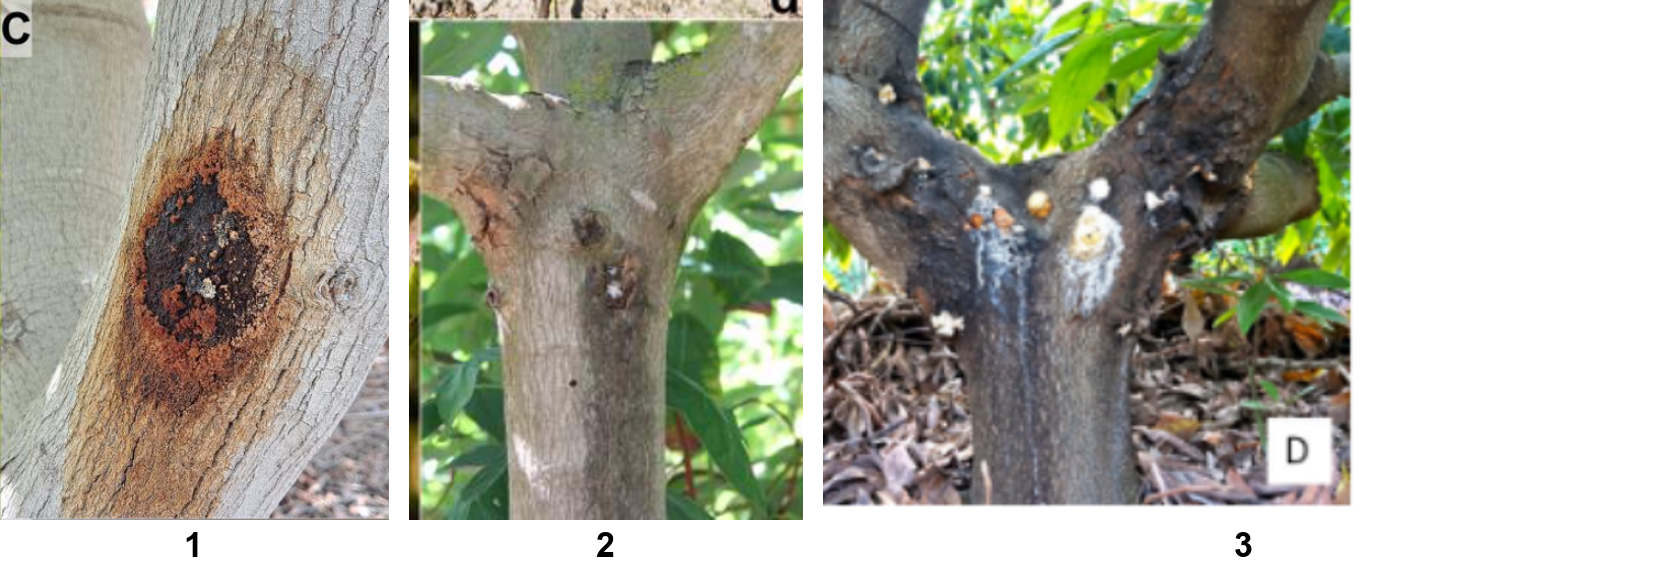
\includegraphics[width=\linewidth,height=0.32\textheight,keepaspectratio]{figuras/lamina1_cancro_exudado.png}
\caption{Cancro con exudado claro en troncos adultos. (1) Centro negro y costroso con puntos blancos y halo pardo rojizo sobre corteza gris (Hernández et al., 2023, Fig. 1C, p. 9). (2) Exudados blanquecinos duros y negros bajo la cruz (Linaldeddu et al., 2026, Fig. 3h, p. 9). (3) Trazos blancos que escurren en la zona de ramificación (Arjona-Girona et al., 2019, Fig. 1D, p. 2). Recortes de artículos CC BY 4.0.}
\end{figure}
\begin{figure}[htbp]
\centering
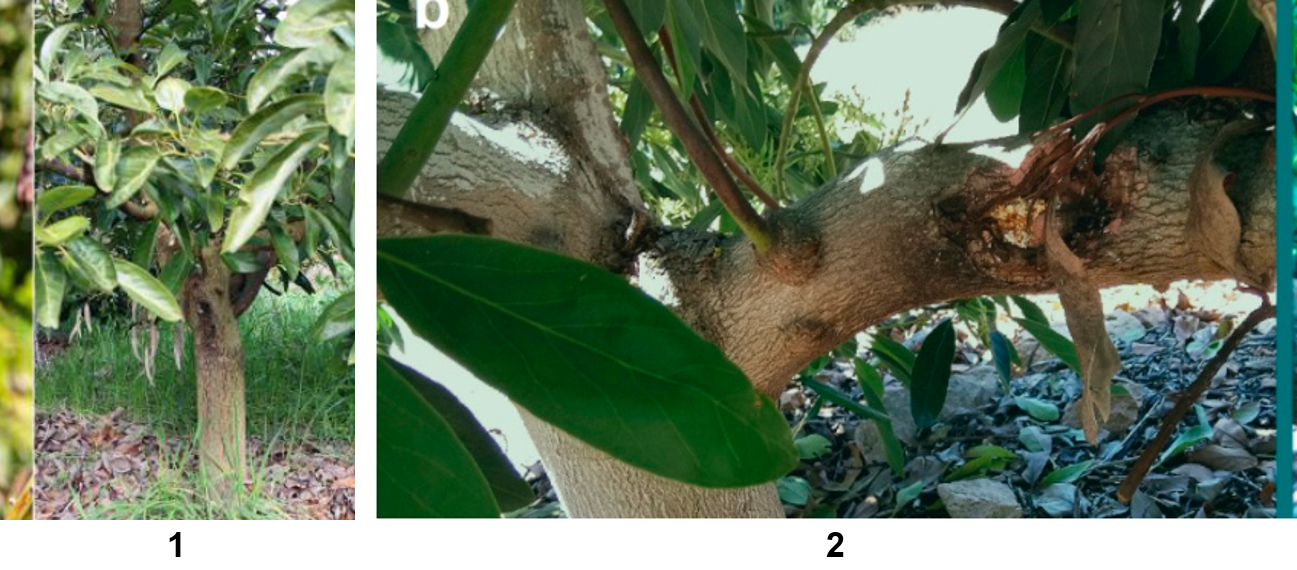
\includegraphics[width=\linewidth,height=0.32\textheight,keepaspectratio]{figuras/lamina2_sangrante_friable.png}
\caption{Necrosis o exudado oscuro y cancro seco. (1) Cancro sangrante oscuro en la base del tronco (Linaldeddu et al., 2026, Fig. 3c, p. 9). (2) Corteza friable y rota cerca del tronco (Valencia et al., 2022, Fig. 1b, p. 3). Recortes de artículos CC BY 4.0.}
\end{figure}
\begin{figure}[htbp]
\centering
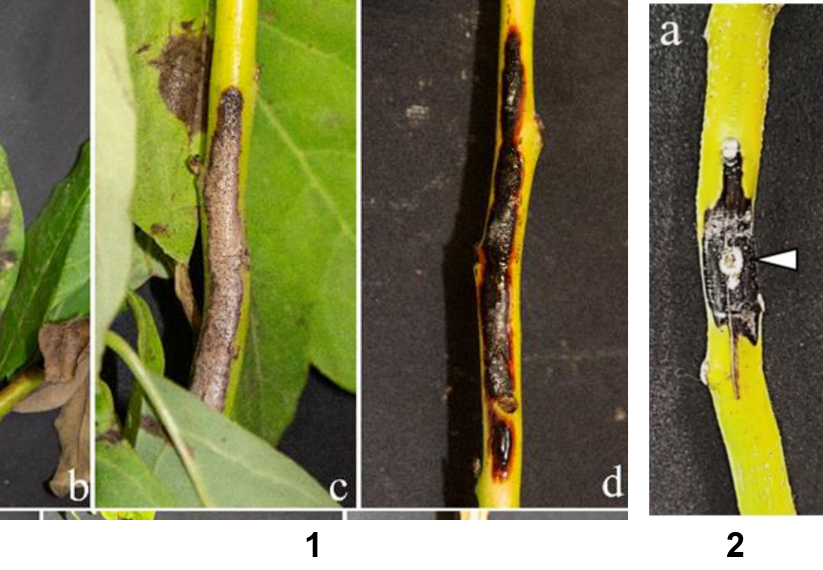
\includegraphics[width=\linewidth,height=0.32\textheight,keepaspectratio]{figuras/lamina3_tallo_joven.png}
\caption{Lesiones en tallos jóvenes. (1) Izquierda: cancro hundido gris pardo (cancro seco); derecha: necrosis negra de corteza (Linaldeddu et al., 2026, Fig. 4c–d, p. 10). (2) Necrosis negra en un tallo inoculado (Rodríguez-Gálvez et al., 2025, Fig. 1a, p. 2). Recortes de artículos CC BY 4.0.}
\end{figure}
\begin{figure}[htbp]
\centering
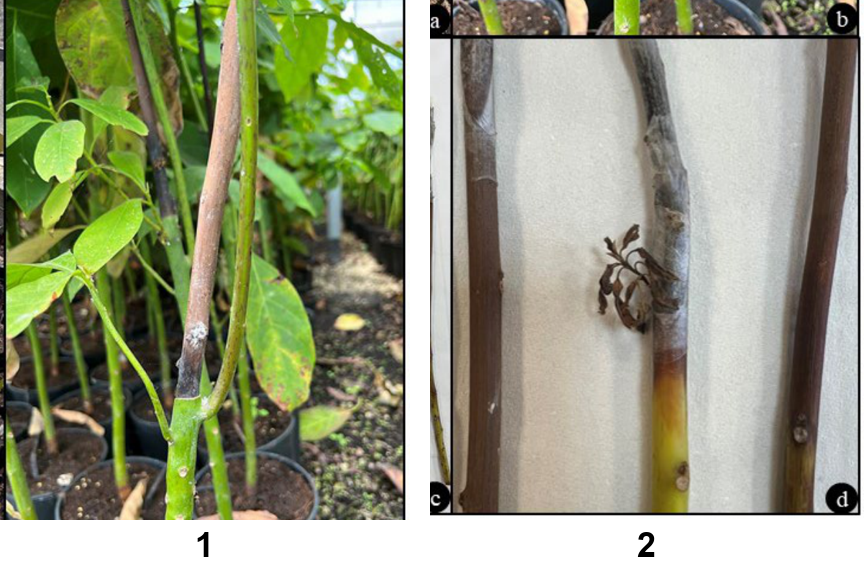
\includegraphics[width=\linewidth,height=0.32\textheight,keepaspectratio]{figuras/lamina4_injerto.png}
\caption{Lesiones que nacen en el injerto de plantas jóvenes: tallo pardo oscuro sobre la variedad y verde amarillento bajo el injerto (Vecchio, Martino, et al., 2026, Fig. 1b y 1d, p. 6). Recorte de un artículo CC BY 4.0.}
\end{figure}
\begin{figure}[htbp]
\centering
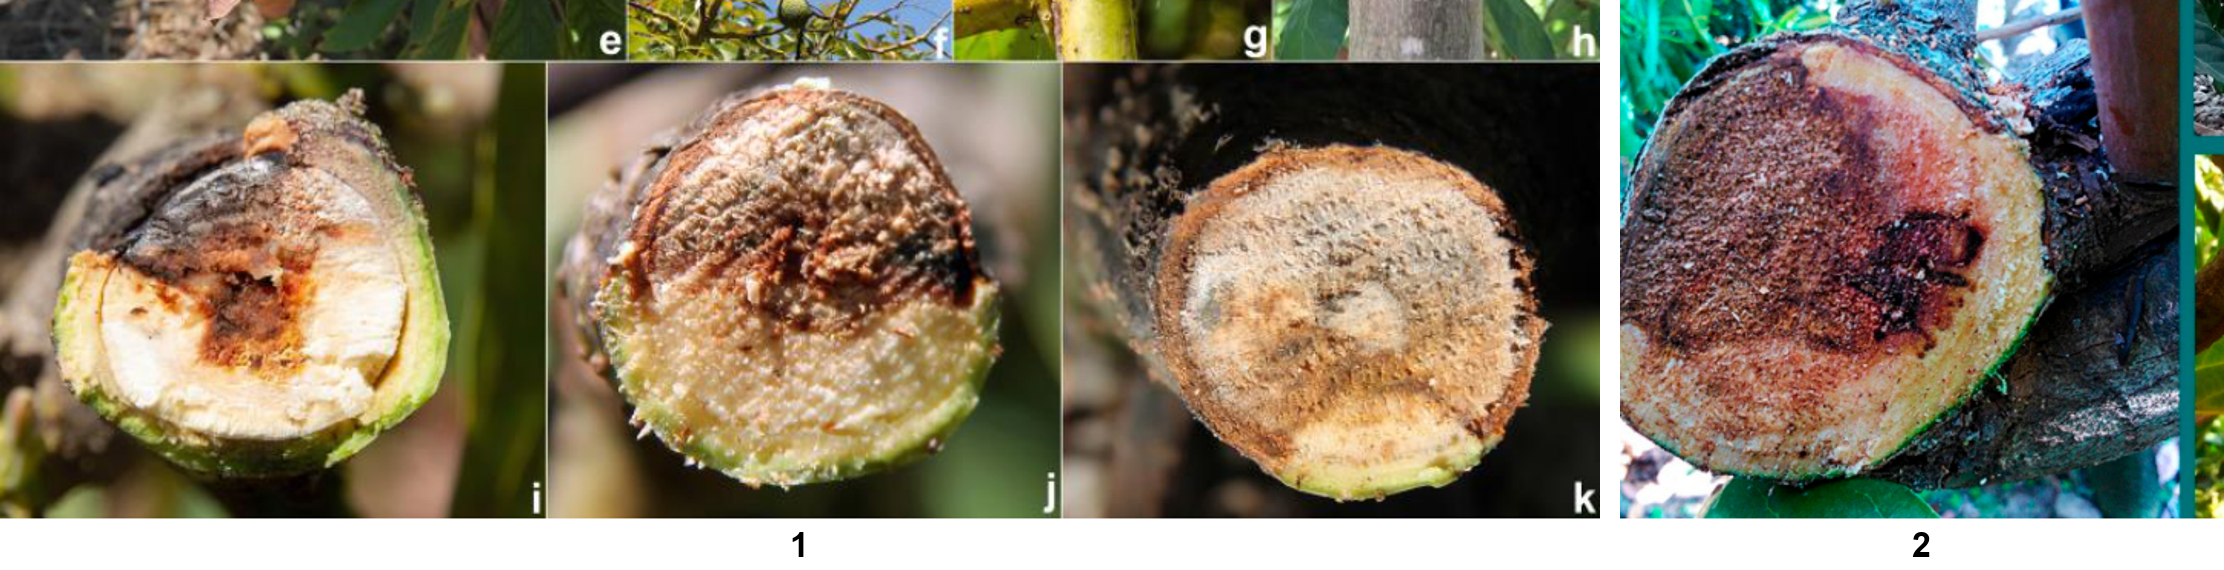
\includegraphics[width=\linewidth,height=0.32\textheight,keepaspectratio]{figuras/lamina5_necrosis_interna.png}
\caption{Lo que la foto externa no muestra: necrosis interna en cortes del tronco (Linaldeddu et al., 2026, Fig. 3i–k, p. 9; Valencia et al., 2022, Fig. 1d, p. 3). Por eso la app debe recomendar confirmar en laboratorio. Recortes de artículos CC BY 4.0.}
\end{figure}
\section{Diccionario de datos}
Las tablas se guardan como CSV en UTF-8 en \nolinkurl{02_tablas}. “Oblig.” indica si el campo es obligatorio.

{\small
\begin{longtable}{|>{\RaggedRight\arraybackslash}p{4.81cm}|>{\RaggedRight\arraybackslash}p{8.27cm}|>{\RaggedRight\arraybackslash}p{1.54cm}|}
\caption{Tabla fincas}\\
\hline
\rowcolor{encabezado}\textbf{Campo} & \textbf{Valores} & \textbf{Oblig.} \\ \hline
\endfirsthead
\hline
\rowcolor{encabezado}\textbf{Campo} & \textbf{Valores} & \textbf{Oblig.} \\ \hline
\endhead
id\_finca & Código de la finca (F01, F02…) & Sí \\ \hline
fecha\_visita & AAAA-MM-DD & Sí \\ \hline
parroquia & Texto & Sí \\ \hline
clima\_observado & soleado / parcialmente nublado / nublado / lluvia & Sí \\ \hline
etapa\_fenologica & floración / cuajado / desarrollo del fruto / cosecha / sin dato & No \\ \hline
variedad, portainjerto & Texto o “sin dato” & No \\ \hline
arboles\_revisados, arboles\_con\_sintomas & Enteros & Sí \\ \hline
consentimiento & sí / no & Sí \\ \hline
\end{longtable}}
{\small
\begin{longtable}{|>{\RaggedRight\arraybackslash}p{4.81cm}|>{\RaggedRight\arraybackslash}p{8.27cm}|>{\RaggedRight\arraybackslash}p{1.54cm}|}
\caption{Tabla arboles}\\
\hline
\rowcolor{encabezado}\textbf{Campo} & \textbf{Valores} & \textbf{Oblig.} \\ \hline
\endfirsthead
\hline
\rowcolor{encabezado}\textbf{Campo} & \textbf{Valores} & \textbf{Oblig.} \\ \hline
\endhead
id\_arbol & F02-A015 & Sí \\ \hline
id\_finca & Código de finca & Sí \\ \hline
grupo\_edad & joven / adulto & Sí \\ \hline
edad\_declarada\_anios & Entero & No \\ \hline
perimetro\_tronco\_cm & Decimal & No \\ \hline
arbol\_con\_sintomas & sí / no & Sí \\ \hline
id\_arbol\_pareado & Código del árbol pareado & No \\ \hline
varios\_tipos\_sintoma & sí / no & Sí \\ \hline
severidad\_arbol & 0 / 1 / 2 / 3 & Sí \\ \hline
liquenes\_musgo & sí / no & Sí \\ \hline
clase\_preliminar\_campo, nota\_campo & Texto & No \\ \hline
\end{longtable}}
{\small
\begin{longtable}{|>{\RaggedRight\arraybackslash}p{4.81cm}|>{\RaggedRight\arraybackslash}p{8.27cm}|>{\RaggedRight\arraybackslash}p{1.54cm}|}
\caption{Tabla lesiones}\\
\hline
\rowcolor{encabezado}\textbf{Campo} & \textbf{Valores} & \textbf{Oblig.} \\ \hline
\endfirsthead
\hline
\rowcolor{encabezado}\textbf{Campo} & \textbf{Valores} & \textbf{Oblig.} \\ \hline
\endhead
id\_lesion & F02-A015-L1 (máximo L3) & Sí \\ \hline
zona & cuello / injerto / fuste / cruz & Sí \\ \hline
cara & N / S / E / O & Sí \\ \hline
longitud\_cm & Decimal & No \\ \hline
\end{longtable}}
{\small
\begin{longtable}{|>{\RaggedRight\arraybackslash}p{4.81cm}|>{\RaggedRight\arraybackslash}p{8.27cm}|>{\RaggedRight\arraybackslash}p{1.54cm}|}
\caption{Tabla imagenes}\\
\hline
\rowcolor{encabezado}\textbf{Campo} & \textbf{Valores} & \textbf{Oblig.} \\ \hline
\endfirsthead
\hline
\rowcolor{encabezado}\textbf{Campo} & \textbf{Valores} & \textbf{Oblig.} \\ \hline
\endhead
id\_imagen & Nombre del archivo sin extensión & Sí \\ \hline
archivo\_original & Nombre que le dio el teléfono & Sí \\ \hline
id\_arbol, id\_lesion & Códigos (lesión vacía si no aplica) & Sí / No \\ \hline
tipo\_foto & ID / GEN / MED / PP / ESC & Sí \\ \hline
angulo & frontal / oblicuo / no aplica & Sí \\ \hline
cara, zona & N/S/E/O; cuello/injerto/fuste/cruz/completa & Sí \\ \hline
fecha\_hora & AAAA-MM-DD hh:mm:ss & Sí \\ \hline
luz & sol directo / sombra / nublado & Sí \\ \hline
corteza\_mojada & sí / no & Sí \\ \hline
telefono, modelo\_telefono & principal / secundario; texto & Sí \\ \hline
ancho\_px, alto\_px & Enteros & Sí \\ \hline
lat\_reducida, lon\_reducida & Decimal con 2 decimales & Sí \\ \hline
estado\_calidad & válida / descartada & Sí \\ \hline
\end{longtable}}
{\small
\begin{longtable}{|>{\RaggedRight\arraybackslash}p{4.81cm}|>{\RaggedRight\arraybackslash}p{8.27cm}|>{\RaggedRight\arraybackslash}p{1.54cm}|}
\caption{Tabla etiquetas}\\
\hline
\rowcolor{encabezado}\textbf{Campo} & \textbf{Valores} & \textbf{Oblig.} \\ \hline
\endfirsthead
\hline
\rowcolor{encabezado}\textbf{Campo} & \textbf{Valores} & \textbf{Oblig.} \\ \hline
\endhead
id\_imagen, sesion & Imagen; 1, 2 o 3 & Sí \\ \hline
etiquetador, fecha, version\_guia & Texto & Sí \\ \hline
etiqueta & sano / exudado\_claro / necrosis\_oscura / cancro\_seco / otra\_alteracion / no\_concluyente & Sí \\ \hline
seguridad & alta / media / baja & Sí \\ \hline
sintoma\_secundario & Una etiqueta o “ninguno” & Sí \\ \hline
caso\_dudoso & Situación aplicada o “ninguno” & Sí \\ \hline
etiqueta\_final & sí / no & Sí \\ \hline
\end{longtable}}
{\small
\begin{longtable}{|>{\RaggedRight\arraybackslash}p{4.81cm}|>{\RaggedRight\arraybackslash}p{8.27cm}|>{\RaggedRight\arraybackslash}p{1.54cm}|}
\caption{Tabla dudas, descartes, niveles y partición}\\
\hline
\rowcolor{encabezado}\textbf{Campo} & \textbf{Valores} & \textbf{Oblig.} \\ \hline
\endfirsthead
\hline
\rowcolor{encabezado}\textbf{Campo} & \textbf{Valores} & \textbf{Oblig.} \\ \hline
\endhead
dudas & id\_imagen, clases\_en\_duda, motivo, decision & Sí \\ \hline
descartes & id\_imagen, motivo, fecha & Sí \\ \hline
niveles & etiqueta, nivel\_A, nivel\_B, nivel\_C & Sí \\ \hline
particion & id\_arbol, id\_grupo, conjunto (desarrollo / prueba / prueba\_externa), pliegue (1 a 5) & Sí \\ \hline
\end{longtable}}
\section{Formatos de campo}
{\small
\begin{longtable}{|>{\RaggedRight\arraybackslash}p{6.06cm}|>{\RaggedRight\arraybackslash}p{8.8cm}|}
\caption{Hoja de finca}\\
\hline
\rowcolor{encabezado}\textbf{Dato} & \textbf{Anotar} \\ \hline
\endfirsthead
\hline
\rowcolor{encabezado}\textbf{Dato} & \textbf{Anotar} \\ \hline
\endhead
Código de finca &  \\ \hline
Fecha y hora de llegada &  \\ \hline
Clima & soleado / parcialmente nublado / nublado / lluvia \\ \hline
Etapa del cultivo &  \\ \hline
Variedad y portainjerto (si los conoce el dueño) &  \\ \hline
Árboles revisados en el recorrido &  \\ \hline
Árboles con síntomas en el tallo &  \\ \hline
Consentimiento firmado & sí / no \\ \hline
\end{longtable}}
{\small
\begin{longtable}{|>{\RaggedRight\arraybackslash}p{6.06cm}|>{\RaggedRight\arraybackslash}p{8.8cm}|}
\caption{Hoja de árbol}\\
\hline
\rowcolor{encabezado}\textbf{Dato} & \textbf{Anotar} \\ \hline
\endfirsthead
\hline
\rowcolor{encabezado}\textbf{Dato} & \textbf{Anotar} \\ \hline
\endhead
Código del árbol (tarjeta) &  \\ \hline
Grupo de edad / edad declarada & joven / adulto; años \\ \hline
¿Tiene síntomas en el tallo? & sí / no \\ \hline
Árbol pareado & código \\ \hline
Lesión 1, 2, 3: zona y cara & cuello / injerto / fuste / cruz; N / S / E / O \\ \hline
Luz / corteza mojada & sol / sombra / nublado; sí / no \\ \hline
Teléfono & principal / secundario \\ \hline
Líquenes o musgo & sí / no \\ \hline
Clase preliminar y nota de campo & p. ej., “poda reciente según el dueño” \\ \hline
\end{longtable}}
\section{Metas y capacidad de captura}
{\small
\begin{longtable}{|>{\RaggedRight\arraybackslash}p{4.81cm}|>{\RaggedRight\arraybackslash}p{3.85cm}|>{\RaggedRight\arraybackslash}p{5.96cm}|}
\caption{Metas por clase}\\
\hline
\rowcolor{encabezado}\textbf{Meta} & \textbf{Árboles distintos} & \textbf{Imágenes válidas (media y primer plano)} \\ \hline
\endfirsthead
\hline
\rowcolor{encabezado}\textbf{Meta} & \textbf{Árboles distintos} & \textbf{Imágenes válidas (media y primer plano)} \\ \hline
\endhead
Mínima & $\geq$ 15 & $\geq$ 50 \\ \hline
Objetivo & $\geq$ 30 & $\geq$ 150 \\ \hline
\end{longtable}}
Estimación con 2 días de captura, 4 fincas, 30 minutos por finca, 1 hora de prueba piloto, 6 minutos por árbol sano y 6 minutos más 5 por lesión por árbol con síntomas (1,5 lesiones en promedio), con un sano pareado por cada enfermo. Los tiempos se reemplazarán por los medidos en la prueba piloto (hoja “Capacidad\_muestreo” del archivo de control).

{\small
\begin{longtable}{|>{\RaggedRight\arraybackslash}p{4.73cm}|>{\RaggedRight\arraybackslash}p{3.02cm}|>{\RaggedRight\arraybackslash}p{2.65cm}|>{\RaggedRight\arraybackslash}p{3.97cm}|}
\caption{Capacidad estimada con 2 días}\\
\hline
\rowcolor{encabezado}\textbf{Escenario (horas útiles por día)} & \textbf{Árboles con síntomas} & \textbf{Árboles sanos} & \textbf{Imágenes de lesión por clase (4 clases)} \\ \hline
\endfirsthead
\hline
\rowcolor{encabezado}\textbf{Escenario (horas útiles por día)} & \textbf{Árboles con síntomas} & \textbf{Árboles sanos} & \textbf{Imágenes de lesión por clase (4 clases)} \\ \hline
\endhead
Pesimista (3 h) & 9 & 9 & $\approx$ 10 \\ \hline
Esperado (4,5 h) & 18 & 18 & $\approx$ 20 \\ \hline
Optimista (6 h) & 27 & 27 & $\approx$ 30 \\ \hline
\end{longtable}}
\textbf{Conclusión:} con 2 días, lo realista es el \textbf{Nivel C} (sano, afectado y otra alteración). El Nivel A (5 clases) requiere unos 4 a 5 días efectivos y el Nivel C unos 2 a 3. Se recomienda pedir 1 o 2 días más o una segunda salida.

\section{Equivalencias con los documentos de soporte}
Este SRS reemplaza la lectura de los documentos de soporte DS-01 a DS-10, que contienen el análisis detallado. Para quien los consulte, estas son las equivalencias de nombres:

{\small
\begin{longtable}{|>{\RaggedRight\arraybackslash}p{8.41cm}|>{\RaggedRight\arraybackslash}p{6.45cm}|}
\caption{Equivalencias de nombres}\\
\hline
\rowcolor{encabezado}\textbf{En este SRS} & \textbf{En los documentos de soporte} \\ \hline
\endfirsthead
\hline
\rowcolor{encabezado}\textbf{En este SRS} & \textbf{En los documentos de soporte} \\ \hline
\endhead
Sano / Cancro con exudado claro / Necrosis o exudado oscuro / Cancro seco / Otra alteración / No concluyente & C0 / C1 / C2 / C3 / C7 / NC \\ \hline
Foto de identificación / general / media / primer plano / con escala & T0 / TG / TM / TP / TE \\ \hline
Cuello / injerto / fuste / cruz & Z1 / Z2 / Z3 / Z4 \\ \hline
RF-01 a RF-28 y RNF-01 a RNF-27 & RD-01 a RD-55 (borrador anterior en el historial) \\ \hline
\end{longtable}}
\section*{Bibliografía}
\addcontentsline{toc}{section}{Bibliografía}
{\small Todas las fuentes forman parte de la carpeta de fuentes recopiladas por el autor.\par}
\begin{list}{}{\leftmargin=1.27cm \itemindent=-1.27cm \itemsep=4pt \parsep=0pt}
\item Ahmed, M., Babaei, M., Jeong, N., Kong, L., \& Gan, Y. (2026). Hybrid loss for robust ripeness classification under noisy labels. \textit{Future Foods, 14}, 101116. \url{https://doi.org/10.1016/j.fufo.2026.101116}
\item Arjona-Girona, I., Ruano-Rosa, D., \& López-Herrera, C. J. (2019). Identification, pathogenicity and distribution of the causal agents of dieback in avocado orchards in Spain. \textit{Spanish Journal of Agricultural Research, 17}(1), e1003. \url{https://doi.org/10.5424/sjar/2019171-13561}
\item Bejarano-Bolívar, A. A., Lamelas, A., Aguirre von Wobeser, E., Sánchez-Rangel, D., Méndez-Bravo, A., Eskalen, A., \& Reverchon, F. (2021). Shifts in the structure of rhizosphere bacterial communities of avocado after Fusarium dieback. \textit{Rhizosphere, 18}, 100333. \url{https://doi.org/10.1016/j.rhisph.2021.100333}
\item Christakakis, P., Papadopoulou, G., Mikos, G., Kalogiannidis, N., Ioannidis, D., Tzovaras, D., \& Pechlivani, E. M. (2024). Smartphone-based citizen science tool for plant disease and insect pest detection using artificial intelligence. \textit{Technologies, 12}(7), 101. \url{https://doi.org/10.3390/technologies12070101}
\item Della Antonia, B., de Oliveira, J., Moreira da Silva, P. P., Biazotto, A. dos M., de Toledo, N. M. V., da Glória, E. M., \& Spoto, M. H. F. (2024). Positive effect of \textit{Lippia sidoides} essential oil associated with carboxymethylcellulose in the control of anthracnose in avocado. \textit{Food Production, Processing and Nutrition, 6}, 39. \url{https://doi.org/10.1186/s43014-023-00209-1}
\item Estrada, J. S., Cetin, N., Sacilik, K., Ulu, B., Ulu, B., \& Auat Cheein, F. (2026). Assessment of avocado water stress using multispectral imaging and deep learning: Toward scalable, cost-effective irrigation monitoring. \textit{Expert Systems with Applications, 326}, 132688. \url{https://doi.org/10.1016/j.eswa.2026.132688}
\item Guirado-Manzano, L., Santamaría-Ortega, J. F., Sarmiento, D., Guirado, E., Pulido-Ruiz, M., de Vicente, A., Fernández-Ortuño, D., Cazorla, F. M., \& Arrebola, E. (2026). Integrated strategies to reduce Botryosphaeriaceae-associated dieback in avocado under Mediterranean climatic stress. \textit{Horticulturae, 12}(6), 673. \url{https://doi.org/10.3390/horticulturae12060673}
\item Hernández, D., García-Pérez, O., Perera, S., González-Carracedo, M. A., Rodríguez-Pérez, A., \& Siverio, F. (2023). Fungal pathogens associated with aerial symptoms of avocado (\textit{Persea americana} Mill.) in Tenerife (Canary Islands, Spain) focused on species of the family Botryosphaeriaceae. \textit{Microorganisms, 11}(3), 585. \url{https://doi.org/10.3390/microorganisms11030585}
\item Iqbal, A., Ahmed, I., Rehman, S., \& Alzahrani, A. S. (2026). Plants disease detection and identification system using AI and computer vision techniques. \textit{PeerJ Computer Science, 12}, e3509. \url{https://doi.org/10.7717/peerj-cs.3509}
\item Kochhar, A., Narang, G., Patel, S., Kaur, H., Singla, C., Pateriya, B., \& Galdelli, A. (2026). A three-tier deep learning framework with mobile application integration for multi-crop disease diagnosis. \textit{Discover Artificial Intelligence, 6}, 358. \url{https://doi.org/10.1007/s44163-026-01062-0}
\item Linaldeddu, B. T., Bregant, C., Muscas, J., Maddau, L., Vecchio, L., Polizzi, G., \& Aiello, D. (2026). Identification and pathogenicity of Botryosphaeriaceae, \textit{Colletotrichum}, and \textit{Phytophthora} species associated with avocado diseases in Italy. \textit{Agriculture, 16}(10), 1035. \url{https://doi.org/10.3390/agriculture16101035}
\item Majdalawieh, M., Martins, C., Radi, M., Alaraj, M., \& Khan, S. (2025). Precision agriculture in the age of AI: A systematic review of machine learning methods for crop disease detection. \textit{Smart Agricultural Technology, 12}, 101491. \url{https://doi.org/10.1016/j.atech.2025.101491}
\item Martinelli, S., Lopes, L., \& Zaina, L. (2024). UX research practices related to long-term UX: A systematic literature review. \textit{Information and Software Technology, 170}, 107431. \url{https://doi.org/10.1016/j.infsof.2024.107431}
\item Möller, H., Slippers, B., \& van den Berg, N. (2025). Branch canker battles: Understanding and managing the Botryosphaeriaceae in avocado. \textit{Phytoparasitica, 53}, 17. \url{https://doi.org/10.1007/s12600-024-01227-6}
\item Ovalle, C., Garcia Jimenez, J., \& Briones Zuñiga, J. (2026). Comparing global and variety-specific ensemble models for avocado maturity prediction with near-infrared. \textit{IAES International Journal of Artificial Intelligence, 15}(3), 2300–2313. \url{https://doi.org/10.11591/ijai.v15.i3.pp2300-2313}
\item Rodríguez-Gálvez, E., Haro-Diaz, C., Maza-Aguirre, S., Canahuire-Castillo, F., Sullón-Saucedo, J., \& Deising, H. B. (2025). \textit{Lasiodiplodia theobromae} disease symptom development in young avocado (\textit{Persea americana} L.) plants depends on the inoculation method. \textit{Tropical Plant Pathology, 50}, 18. \url{https://doi.org/10.1007/s40858-025-00700-9}
\item Saini, Y., Somani, V., \& Khatri, N. (2026). Critical analysis of advanced machine learning and deep learning models for crop disease detection: Challenges, innovations, and future directions. \textit{Franklin Open, 15}, 100584. \url{https://doi.org/10.1016/j.fraope.2026.100584}
\item Valencia, A. L., Saavedra-Torrico, J., Rosales, I. M., Mártiz, J., Retamales, A., Link, A., \& Gil, P. M. (2022). Unveiling the predisposing factors for the development of branch canker and dieback in avocado: A case of study in Chilean orchards. \textit{Horticulturae, 8}(12), 1121. \url{https://doi.org/10.3390/horticulturae8121121}
\item Vecchio, L., Arrebola, E., Polizzi, G., \& Vitale, A. (2026). Ecofriendly management of anthracnose on avocado caused by \textit{Colletotrichum perseae} in the Mediterranean basin. \textit{JSFA Reports}. Publicación anticipada en línea. \url{https://doi.org/10.1002/jsf2.70088}
\item Vecchio, L., Martino, I., Guarnaccia, V., Polizzi, G., \& Aiello, D. (2026). \textit{Colletotrichum perseae} and \textit{Colletotrichum gloeosporioides} sensu strictu causing stem lesion and dieback in avocado in Italy. \textit{Horticulturae, 12}(1), 111. \url{https://doi.org/10.3390/horticulturae12010111}
\item Xavier, P., Rodrigues, P. M., \& Silva, C. L. M. (2024). Shelf-life management and ripening assessment of `Hass\textquotesingle{} avocado (\textit{Persea americana}) using deep learning approaches. \textit{Foods, 13}(8), 1150. \url{https://doi.org/10.3390/foods13081150}
\item Yuan, L., Li, W., Yue, J., Li, Z., Zhao, Y., Li, Q., Feng, W., \& Kou, G. (2026). A review of cattle behavior recognition methods based on computer vision and deep learning. \textit{Smart Agricultural Technology, 14}, 101867. \url{https://doi.org/10.1016/j.atech.2026.101867}
\end{list}
\end{document}
